%%%%%%%%%%%%%%%%%%%%%%%%%%%%%%%%%%%%%%%%%
% The Legrand Orange Book
% LaTeX Template
% Version 2.1 (14/11/15)
%
% This template has been downloaded from:
% http://www.LaTeXTemplates.com
%
% Mathias Legrand (legrand.mathias@gmail.com) with modifications by:
% Vel (vel@latextemplates.com)
%
% License:
% CC BY-NC-SA 3.0 (http://creativecommons.org/licenses/by-nc-sa/3.0/)
%
% Compiling this template:
% This template uses biber for its bibliography and makeindex for its index.
% When you first open the template, compile it from the command line with the 
% commands below to make sure your LaTeX distribution is configured correctly:
%
% 1) pdflatex main
% 2) makeindex main.idx -s StyleInd.ist
% 3) biber main
% 4) pdflatex main x 2
%
% After this, when you wish to update the bibliography/index use the appropriate
% command above and make sure to compile with pdflatex several times 
% afterwards to propagate your changes to the document.
%
% This template also uses a number of packages which may need to be
% updated to the newest versions for the template to compile. It is strongly
% recommended you update your LaTeX distribution if you have any
% compilation errors.
%
% Important note:
% Chapter heading images should have a 2:1 width:height ratio,
% e.g. 920px width and 460px height.
%
%%%%%%%%%%%%%%%%%%%%%%%%%%%%%%%%%%%%%%%%%

%----------------------------------------------------------------------------------------
%	PACKAGES AND OTHER DOCUMENT CONFIGURATIONS
%----------------------------------------------------------------------------------------

\documentclass[11pt,fleqn]{book} % Default font size and left-justified equations
\usepackage[dvipsnames]{xcolor}
\usepackage{wrapfig}
\usepackage{listings}
\usepackage{textcomp}
\usepackage{smartdiagram}
\usepackage{texshade}
%----------------------------------------------------------------------------------------
\lstset{frame=tb,
  language=Bash,
  aboveskip=3mm,
  belowskip=3mm,
  showstringspaces=false,
  columns=flexible,
  basicstyle={\small\ttfamily},
  numbers=none,
  numberstyle=\tiny\color{black},
  keywordstyle=\color{black},
  commentstyle=\color{black},
  stringstyle=\color{black},
  breaklines=true,
  breakatwhitespace=true,
  tabsize=3
}
%%%%%%%%%%%%%%%%%%%%%%%%%%%%%%%%%%%%%%%%%
% The Legrand Orange Book
% Structural Definitions File
% Version 2.0 (9/2/15)
%
% Original author:
% Mathias Legrand (legrand.mathias@gmail.com) with modifications by:
% Vel (vel@latextemplates.com)
% 
% This file has been downloaded from:
% http://www.LaTeXTemplates.com
%
% License:
% CC BY-NC-SA 3.0 (http://creativecommons.org/licenses/by-nc-sa/3.0/)
%
%%%%%%%%%%%%%%%%%%%%%%%%%%%%%%%%%%%%%%%%%

%----------------------------------------------------------------------------------------
%	VARIOUS REQUIRED PACKAGES AND CONFIGURATIONS
%----------------------------------------------------------------------------------------

\usepackage[top=3cm,bottom=3cm,left=3cm,right=3cm,headsep=10pt,a4paper]{geometry} % Page margins

\usepackage{graphicx} % Required for including pictures
\graphicspath{{Pictures/}} % Specifies the directory where pictures are stored

\usepackage{lipsum} % Inserts dummy text

\usepackage{tikz} % Required for drawing custom shapes

\usepackage[english]{babel} % English language/hyphenation

\usepackage{enumitem} % Customize lists
\setlist{nolistsep} % Reduce spacing between bullet points and numbered lists

\usepackage{booktabs} % Required for nicer horizontal rules in tables

\usepackage{xcolor} % Required for specifying colors by name
\definecolor{ocre}{RGB}{243,102,25} % Define the orange color used for highlighting throughout the book
\definecolor{red}{RGB}{255,25,25}
%----------------------------------------------------------------------------------------
%	FONTS
%----------------------------------------------------------------------------------------
\usepackage[lighttt]{lmodern}
\usepackage{bold-extra}
\usepackage{avant} % Use the Avantgarde font for headings
%\usepackage{times} % Use the Times font for headings
\usepackage{mathptmx} % Use the Adobe Times Roman as the default text font together with math symbols from the Sym­bol, Chancery and Com­puter Modern fonts

\usepackage{microtype} % Slightly tweak font spacing for aesthetics
\usepackage[utf8]{inputenc} % Required for including letters with accents
\usepackage[T1]{fontenc} % Use 8-bit encoding that has 256 glyphs

\usepackage{wrapfig}
\usepackage{listings}
\usepackage{textcomp}
\usepackage{smartdiagram}
\usepackage{texshade}
%----------------------------------------------------------------------------------------
\lstset{frame=tb,
  language=Bash,
  aboveskip=3mm,
  belowskip=3mm,
  showstringspaces=false,
  columns=flexible,
  basicstyle={\small\ttfamily},
  numbers=none,
  numberstyle=\tiny\color{black},
  keywordstyle=\color{black},
  commentstyle=\color{black},
  stringstyle=\color{black},
  breaklines=true,
  breakatwhitespace=true,
  tabsize=3
}

%----------------------------------------------------------------------------------------
%	BIBLIOGRAPHY AND INDEX
%----------------------------------------------------------------------------------------

% \usepackage[style=alphabetic,citestyle=numeric,sorting=nyt,sortcites=true,autopunct=true,babel=hyphen,hyperref=true,abbreviate=false,backref=true,backend=biber]{biblatex}
\usepackage{biblatex}
\addbibresource{bibliography.bib} % BibTeX bibliography file
% \defbibheading{bibempty}{}

\usepackage{calc} % For simpler calculation - used for spacing the index letter headings correctly
\usepackage{makeidx} % Required to make an index
\makeindex % Tells LaTeX to create the files required for indexing

%----------------------------------------------------------------------------------------
%	MAIN TABLE OF CONTENTS
%----------------------------------------------------------------------------------------

\usepackage{titletoc} % Required for manipulating the table of contents

\contentsmargin{0cm} % Removes the default margin

% Part text styling
\titlecontents{part}[0cm]
{\addvspace{20pt}\centering\large\bfseries}
{}
{}
{}

% Chapter text styling
\titlecontents{chapter}[1.25cm] % Indentation
{\addvspace{12pt}\large\sffamily\bfseries} % Spacing and font options for chapters
{\color{ocre!60}\contentslabel[\Large\thecontentslabel]{1.25cm}\color{ocre}} % Chapter number
{\color{ocre}}  
{\color{ocre!60}\normalsize\;\titlerule*[.5pc]{.}\;\thecontentspage} % Page number

% Section text styling
\titlecontents{section}[1.25cm] % Indentation
{\addvspace{3pt}\sffamily\bfseries} % Spacing and font options for sections
{\contentslabel[\thecontentslabel]{1.25cm}} % Section number
{}
{\hfill\color{black}\thecontentspage} % Page number
[]

% Subsection text styling
\titlecontents{subsection}[1.25cm] % Indentation
{\addvspace{1pt}\sffamily\small} % Spacing and font options for subsections
{\contentslabel[\thecontentslabel]{1.25cm}} % Subsection number
{}
{\ \titlerule*[.5pc]{.}\;\thecontentspage} % Page number
[]

% List of figures
\titlecontents{figure}[0em]
{\addvspace{-5pt}\sffamily}
{\thecontentslabel\hspace*{1em}}
{}
{\ \titlerule*[.5pc]{.}\;\thecontentspage}
[]

% List of tables
\titlecontents{table}[0em]
{\addvspace{-5pt}\sffamily}
{\thecontentslabel\hspace*{1em}}
{}
{\ \titlerule*[.5pc]{.}\;\thecontentspage}
[]

%----------------------------------------------------------------------------------------
%	MINI TABLE OF CONTENTS IN PART HEADS
%----------------------------------------------------------------------------------------

% Chapter text styling
\titlecontents{lchapter}[0em] % Indenting
{\addvspace{15pt}\large\sffamily\bfseries} % Spacing and font options for chapters
{\color{ocre}\contentslabel[\Large\thecontentslabel]{1.25cm}\color{ocre}} % Chapter number
{}  
{\color{ocre}\normalsize\sffamily\bfseries\;\titlerule*[.5pc]{.}\;\thecontentspage} % Page number

% Section text styling
\titlecontents{lsection}[0em] % Indenting
{\sffamily\small} % Spacing and font options for sections
{\contentslabel[\thecontentslabel]{1.25cm}} % Section number
{}
{}

% Subsection text styling
\titlecontents{lsubsection}[.5em] % Indentation
{\normalfont\footnotesize\sffamily} % Font settings
{}
{}
{}

%----------------------------------------------------------------------------------------
%	PAGE HEADERS
%----------------------------------------------------------------------------------------

\usepackage{fancyhdr} % Required for header and footer configuration

\pagestyle{fancy}
\renewcommand{\chaptermark}[1]{\markboth{\sffamily\normalsize\bfseries\chaptername\ \thechapter.\ #1}{}} % Chapter text font settings
\renewcommand{\sectionmark}[1]{\markright{\sffamily\normalsize\thesection\hspace{5pt}#1}{}} % Section text font settings
\fancyhf{} \fancyhead[LE,RO]{\sffamily\normalsize\thepage} % Font setting for the page number in the header
\fancyhead[LO]{\rightmark} % Print the nearest section name on the left side of odd pages
\fancyhead[RE]{\leftmark} % Print the current chapter name on the right side of even pages
\renewcommand{\headrulewidth}{0.5pt} % Width of the rule under the header
\addtolength{\headheight}{2.5pt} % Increase the spacing around the header slightly
\renewcommand{\footrulewidth}{0pt} % Removes the rule in the footer
\fancypagestyle{plain}{\fancyhead{}\renewcommand{\headrulewidth}{0pt}} % Style for when a plain pagestyle is specified

% Removes the header from odd empty pages at the end of chapters
\makeatletter
\renewcommand{\cleardoublepage}{
\clearpage\ifodd\c@page\else
\hbox{}
\vspace*{\fill}
\thispagestyle{empty}
\newpage
\fi}

%----------------------------------------------------------------------------------------
%	THEOREM STYLES
%----------------------------------------------------------------------------------------

\usepackage{amsmath,amsfonts,amssymb,amsthm} % For math equations, theorems, symbols, etc

\newcommand{\intoo}[2]{\mathopen{]}#1\,;#2\mathclose{[}}
\newcommand{\ud}{\mathop{\mathrm{{}d}}\mathopen{}}
\newcommand{\intff}[2]{\mathopen{[}#1\,;#2\mathclose{]}}
\newtheorem{notation}{Notation}[chapter]

% Boxed/framed environments
\newtheoremstyle{ocrenumbox}% % Theorem style name
{0pt}% Space above
{0pt}% Space below
{\normalfont}% % Body font
{}% Indent amount
{\small\bf\sffamily\color{ocre}}% % Theorem head font
{\;}% Punctuation after theorem head
{0.25em}% Space after theorem head
{\small\sffamily\color{ocre}\thmname{#1}\nobreakspace\thmnumber{\@ifnotempty{#1}{}\@upn{#2}}% Theorem text (e.g. Theorem 2.1)
\thmnote{\nobreakspace\the\thm@notefont\sffamily\bfseries\color{black}---\nobreakspace#3.}} % Optional theorem note
\renewcommand{\qedsymbol}{$\blacksquare$}% Optional qed square

\newtheoremstyle{blacknumex}% Theorem style name
{5pt}% Space above
{5pt}% Space below
{\normalfont}% Body font
{} % Indent amount
{\small\bf\sffamily}% Theorem head font
{\;}% Punctuation after theorem head
{0.25em}% Space after theorem head
{\small\sffamily{\tiny\ensuremath{\blacksquare}}\nobreakspace\thmname{#1}\nobreakspace\thmnumber{\@ifnotempty{#1}{}\@upn{#2}}% Theorem text (e.g. Theorem 2.1)
\thmnote{\nobreakspace\the\thm@notefont\sffamily\bfseries---\nobreakspace#3.}}% Optional theorem note

\newtheoremstyle{blacknumbox} % Theorem style name
{0pt}% Space above
{0pt}% Space below
{\normalfont}% Body font
{}% Indent amount
{\small\bf\sffamily}% Theorem head font
{\;}% Punctuation after theorem head
{0.25em}% Space after theorem head
{\small\sffamily\thmname{#1}\nobreakspace\thmnumber{\@ifnotempty{#1}{}\@upn{#2}}% Theorem text (e.g. Theorem 2.1)
\thmnote{\nobreakspace\the\thm@notefont\sffamily\bfseries---\nobreakspace#3.}}% Optional theorem note

% Non-boxed/non-framed environments
\newtheoremstyle{ocrenum}% % Theorem style name
{5pt}% Space above
{5pt}% Space below
{\normalfont}% % Body font
{}% Indent amount
{\small\bf\sffamily\color{ocre}}% % Theorem head font
{\;}% Punctuation after theorem head
{0.25em}% Space after theorem head
{\small\sffamily\color{ocre}\thmname{#1}\nobreakspace\thmnumber{\@ifnotempty{#1}{}\@upn{#2}}% Theorem text (e.g. Theorem 2.1)
\thmnote{\nobreakspace\the\thm@notefont\sffamily\bfseries\color{black}---\nobreakspace#3.}} % Optional theorem note
\renewcommand{\qedsymbol}{$\blacksquare$}% Optional qed square
\makeatother

% Defines the theorem text style for each type of theorem to one of the three styles above
\newcounter{dummy} 
\numberwithin{dummy}{section}
\theoremstyle{ocrenumbox}
\newtheorem{theoremeT}[dummy]{Theorem}
\newtheorem{problem}{Problem}[chapter]
\newtheorem{exerciseT}{Exercise}[chapter]
\theoremstyle{blacknumex}
\newtheorem{exampleT}{Example}[chapter]
\theoremstyle{blacknumbox}
\newtheorem{vocabulary}{Vocabulary}[chapter]
\newtheorem{definitionT}{Definition}[section]
\newtheorem{corollaryT}[dummy]{Corollary}
\theoremstyle{ocrenum}
\newtheorem{proposition}[dummy]{Proposition}

%----------------------------------------------------------------------------------------
%	DEFINITION OF COLORED BOXES
%----------------------------------------------------------------------------------------

\RequirePackage[framemethod=default]{mdframed} % Required for creating the theorem, definition, exercise and corollary boxes

% Theorem box
\newmdenv[skipabove=7pt,
skipbelow=7pt,
backgroundcolor=black!5,
linecolor=ocre,
innerleftmargin=5pt,
innerrightmargin=5pt,
innertopmargin=5pt,
leftmargin=0cm,
rightmargin=0cm,
innerbottommargin=5pt]{tBox}

% Exercise box	  
\newmdenv[skipabove=7pt,
skipbelow=7pt,
rightline=false,
leftline=true,
topline=false,
bottomline=false,
backgroundcolor=ocre!10,
linecolor=ocre,
innerleftmargin=5pt,
innerrightmargin=5pt,
innertopmargin=5pt,
innerbottommargin=5pt,
leftmargin=0cm,
rightmargin=0cm,
linewidth=4pt]{eBox}	

% Definition box
\newmdenv[skipabove=7pt,
skipbelow=7pt,
rightline=false,
leftline=true,
topline=false,
bottomline=false,
linecolor=ocre,
innerleftmargin=5pt,
innerrightmargin=5pt,
innertopmargin=0pt,
leftmargin=0cm,
rightmargin=0cm,
linewidth=4pt,
innerbottommargin=0pt]{dBox}	

% Corollary box
\newmdenv[skipabove=7pt,
skipbelow=7pt,
rightline=false,
leftline=true,
topline=false,
bottomline=false,
linecolor=gray,
backgroundcolor=black!5,
innerleftmargin=5pt,
innerrightmargin=5pt,
innertopmargin=5pt,
leftmargin=0cm,
rightmargin=0cm,
linewidth=4pt,
innerbottommargin=5pt]{cBox}

% Creates an environment for each type of theorem and assigns it a theorem text style from the "Theorem Styles" section above and a colored box from above
\newenvironment{theorem}{\begin{tBox}\begin{theoremeT}}{\end{theoremeT}\end{tBox}}
\newenvironment{exercise}{\begin{eBox}\begin{exerciseT}}{\hfill{\color{ocre}\tiny\ensuremath{\blacksquare}}\end{exerciseT}\end{eBox}}				  
\newenvironment{definition}{\begin{dBox}\begin{definitionT}}{\end{definitionT}\end{dBox}}	
\newenvironment{example}{\begin{exampleT}}{\hfill{\tiny\ensuremath{\blacksquare}}\end{exampleT}}		
\newenvironment{corollary}{\begin{cBox}\begin{corollaryT}}{\end{corollaryT}\end{cBox}}	

%----------------------------------------------------------------------------------------
%	REMARK ENVIRONMENT
%----------------------------------------------------------------------------------------

\newenvironment{remark}{\par\vspace{10pt}\small % Vertical white space above the remark and smaller font size
\begin{list}{}{
\leftmargin=35pt % Indentation on the left
\rightmargin=25pt}\item\ignorespaces % Indentation on the right
\makebox[-2.5pt]{\begin{tikzpicture}[overlay]
\node[draw=ocre!60,line width=1pt,circle,fill=ocre!25,font=\sffamily\bfseries,inner sep=2pt,outer sep=0pt] at (-15pt,0pt){\textcolor{ocre}{R}};\end{tikzpicture}} % Orange R in a circle
\advance\baselineskip -1pt}{\end{list}\vskip5pt} % Tighter line spacing and white space after remark

%----------------------------------------------------------------------------------------
% WARNING ENVIRONMENT
%----------------------------------------------------------------------------------------

\newenvironment{warning}{\par\vspace{10pt}\small % Vertical white space above the remark and smaller font size
\begin{list}{}{
\leftmargin=35pt % Indentation on the left
\rightmargin=25pt}\item\ignorespaces % Indentation on the right
\makebox[-2.5pt]{\begin{tikzpicture}[overlay]
\node[draw=red!60,line width=1pt,circle,fill=red!25,font=\sffamily\bfseries,inner sep=2pt,outer sep=0pt] at (-15pt,0pt){\textcolor{red}{W}};\end{tikzpicture}} % Orange R in a circle
\advance\baselineskip -1pt}{\end{list}\vskip5pt} % Tighter line spacing and white space after remark

%----------------------------------------------------------------------------------------
%	SECTION NUMBERING IN THE MARGIN
%----------------------------------------------------------------------------------------

\makeatletter
\renewcommand{\@seccntformat}[1]{\llap{\textcolor{ocre}{\csname the#1\endcsname}\hspace{1em}}}                    
\renewcommand{\section}{\@startsection{section}{1}{\z@}
{-4ex \@plus -1ex \@minus -.4ex}
{1ex \@plus.2ex }
{\normalfont\large\sffamily\bfseries}}
\renewcommand{\subsection}{\@startsection {subsection}{2}{\z@}
{-3ex \@plus -0.1ex \@minus -.4ex}
{0.5ex \@plus.2ex }
{\normalfont\sffamily\bfseries}}
\renewcommand{\subsubsection}{\@startsection {subsubsection}{3}{\z@}
{-2ex \@plus -0.1ex \@minus -.2ex}
{.2ex \@plus.2ex }
{\normalfont\small\sffamily\bfseries}}                        
\renewcommand\paragraph{\@startsection{paragraph}{4}{\z@}
{-2ex \@plus-.2ex \@minus .2ex}
{.1ex}
{\normalfont\small\sffamily\bfseries}}

%----------------------------------------------------------------------------------------
%	PART HEADINGS
%----------------------------------------------------------------------------------------

% numbered part in the table of contents
\newcommand{\@mypartnumtocformat}[2]{%
\setlength\fboxsep{0pt}%
\noindent\colorbox{ocre!20}{\strut\parbox[c][.7cm]{\ecart}{\color{ocre!70}\Large\sffamily\bfseries\centering#1}}\hskip\esp\colorbox{ocre!40}{\strut\parbox[c][.7cm]{\linewidth-\ecart-\esp}{\Large\sffamily\centering#2}}}%
%%%%%%%%%%%%%%%%%%%%%%%%%%%%%%%%%%
% unnumbered part in the table of contents
\newcommand{\@myparttocformat}[1]{%
\setlength\fboxsep{0pt}%
\noindent\colorbox{ocre!40}{\strut\parbox[c][.7cm]{\linewidth}{\Large\sffamily\centering#1}}}%
%%%%%%%%%%%%%%%%%%%%%%%%%%%%%%%%%%
\newlength\esp
\setlength\esp{4pt}
\newlength\ecart
\setlength\ecart{1.2cm-\esp}
\newcommand{\thepartimage}{}%
\newcommand{\partimage}[1]{\renewcommand{\thepartimage}{#1}}%
\def\@part[#1]#2{%
\ifnum \c@secnumdepth >-2\relax%
\refstepcounter{part}%
\addcontentsline{toc}{part}{\texorpdfstring{\protect\@mypartnumtocformat{\thepart}{#1}}{\partname~\thepart\ ---\ #1}}
\else%
\addcontentsline{toc}{part}{\texorpdfstring{\protect\@myparttocformat{#1}}{#1}}%
\fi%
\startcontents%
\markboth{}{}%
{\thispagestyle{empty}%
\begin{tikzpicture}[remember picture,overlay]%
\node at (current page.north west){\begin{tikzpicture}[remember picture,overlay]%	
\fill[ocre!20](0cm,0cm) rectangle (\paperwidth,-\paperheight);
\node[anchor=north] at (4cm,-3.25cm){\color{ocre!40}\fontsize{220}{100}\sffamily\bfseries\@Roman\c@part}; 
\node[anchor=south east] at (\paperwidth-1cm,-\paperheight+1cm){\parbox[t][][t]{8.5cm}{
\printcontents{l}{0}{\setcounter{tocdepth}{1}}%
}};
\node[anchor=north east] at (\paperwidth-1.5cm,-3.25cm){\parbox[t][][t]{15cm}{\strut\raggedleft\color{white}\fontsize{30}{30}\sffamily\bfseries#2}};
\end{tikzpicture}};
\end{tikzpicture}}%
\@endpart}
\def\@spart#1{%
\startcontents%
\phantomsection
{\thispagestyle{empty}%
\begin{tikzpicture}[remember picture,overlay]%
\node at (current page.north west){\begin{tikzpicture}[remember picture,overlay]%	
\fill[ocre!20](0cm,0cm) rectangle (\paperwidth,-\paperheight);
\node[anchor=north east] at (\paperwidth-1.5cm,-3.25cm){\parbox[t][][t]{15cm}{\strut\raggedleft\color{white}\fontsize{30}{30}\sffamily\bfseries#1}};
\end{tikzpicture}};
\end{tikzpicture}}
\addcontentsline{toc}{part}{\texorpdfstring{%
\setlength\fboxsep{0pt}%
\noindent\protect\colorbox{ocre!40}{\strut\protect\parbox[c][.7cm]{\linewidth}{\Large\sffamily\protect\centering #1\quad\mbox{}}}}{#1}}%
\@endpart}
\def\@endpart{\vfil\newpage
\if@twoside
\if@openright
\null
\thispagestyle{empty}%
\newpage
\fi
\fi
\if@tempswa
\twocolumn
\fi}

%----------------------------------------------------------------------------------------
%	CHAPTER HEADINGS
%----------------------------------------------------------------------------------------

\newcommand{\thechapterimage}{}%
\newcommand{\chapterimage}[1]{\renewcommand{\thechapterimage}{#1}}%
\def\@makechapterhead#1{%
{\parindent \z@ \raggedright \normalfont
\ifnum \c@secnumdepth >\m@ne
\if@mainmatter
\begin{tikzpicture}[remember picture,overlay]
\node at (current page.north west)
{\begin{tikzpicture}[remember picture,overlay]
\node[anchor=north west,inner sep=0pt] at (0,0) {\includegraphics[width=\paperwidth]{\thechapterimage}};
\draw[anchor=west] (\Gm@lmargin,-9cm) node [line width=2pt,rounded corners=15pt,draw=ocre,fill=white,fill opacity=0.5,inner sep=15pt]{\strut\makebox[22cm]{}};
\draw[anchor=west] (\Gm@lmargin+.3cm,-9cm) node {\huge\sffamily\bfseries\color{black}\thechapter. #1\strut};
\end{tikzpicture}};
\end{tikzpicture}
\else
\begin{tikzpicture}[remember picture,overlay]
\node at (current page.north west)
{\begin{tikzpicture}[remember picture,overlay]
\node[anchor=north west,inner sep=0pt] at (0,0) {\includegraphics[width=\paperwidth]{\thechapterimage}};
\draw[anchor=west] (\Gm@lmargin,-9cm) node [line width=2pt,rounded corners=15pt,draw=ocre,fill=white,fill opacity=0.5,inner sep=15pt]{\strut\makebox[22cm]{}};
\draw[anchor=west] (\Gm@lmargin+.3cm,-9cm) node {\huge\sffamily\bfseries\color{black}#1\strut};
\end{tikzpicture}};
\end{tikzpicture}
\fi\fi\par\vspace*{270\p@}}}

%-------------------------------------------

\def\@makeschapterhead#1{%
\begin{tikzpicture}[remember picture,overlay]
\node at (current page.north west)
{\begin{tikzpicture}[remember picture,overlay]
\node[anchor=north west,inner sep=0pt] at (0,0) {\includegraphics[width=\paperwidth]{\thechapterimage}};
\draw[anchor=west] (\Gm@lmargin,-9cm) node [line width=2pt,rounded corners=15pt,draw=ocre,fill=white,fill opacity=0.5,inner sep=15pt]{\strut\makebox[22cm]{}};
\draw[anchor=west] (\Gm@lmargin+.3cm,-9cm) node {\huge\sffamily\bfseries\color{black}#1\strut};
\end{tikzpicture}};
\end{tikzpicture}
\par\vspace*{270\p@}}
\makeatother

%----------------------------------------------------------------------------------------
%	HYPERLINKS IN THE DOCUMENTS
%----------------------------------------------------------------------------------------

\usepackage{hyperref}
\hypersetup{hidelinks,backref=true,pagebackref=true,hyperindex=true,colorlinks=false,breaklinks=true,urlcolor= ocre,bookmarks=true,bookmarksopen=false,pdftitle={Title},pdfauthor={Author}}
\usepackage{bookmark}
\bookmarksetup{
open,
numbered,
addtohook={%
\ifnum\bookmarkget{level}=0 % chapter
\bookmarksetup{bold}%
\fi
\ifnum\bookmarkget{level}=-1 % part
\bookmarksetup{color=ocre,bold}%
\fi
}
} % Insert the commands.tex file which contains the majority of the structure behind the template


\newcommand{\GeneCount}{{\color{Red} Gene Count }}
\newcommand{\JunctionMake}{{\color{Blue} Junction Make }}
\newcommand{\BlastQuery}{{\color{ForestGreen} Blast Query }}
\newcommand{\ReadDepth}{{\color{Bittersweet} Read Depth }}
\newcommand{\DEEPN}{\textbf{DEEPN }}

\begin{document}

%----------------------------------------------------------------------------------------
%	TITLE PAGE
%----------------------------------------------------------------------------------------

\begingroup
\thispagestyle{empty}
\begin{tikzpicture}[remember picture,overlay]
\coordinate [below=10.5cm] (midpoint) at (current page.north);
\node at (current page.north west)
{\begin{tikzpicture}[remember picture,overlay]
\node[anchor=north west,inner sep=0pt] at (0,0) {
\includegraphics[width=\paperwidth]{background}}; % Background image
\draw[anchor=north] (midpoint) node [fill=ocre!30!white,fill opacity=0.6,text opacity=1,inner sep=1cm]{\Huge\centering\bfseries\sffamily\parbox[c][][t]{0.9\paperwidth}{\centering DEEPN Methods v1.1\\ % Book title
\textnormal{\sffamily\Large \textbf{D}ynamic \textbf{E}nrichment for \textbf{E}valuation of \textbf{P}rotein \textbf{N}etworks}\\[20pt] % Subtitle
{\huge Working With Yeast \hfill{Illumina Data Processing  }}\\[10pt]
{\Large Tabitha Peterson \hfill{Venkatramanan Krishnamani}}\\[-1pt]
{\Large Natasha Pashkova \hfill{Mark Stamnes}}\\[-1pt]
{\Large \hfill{Robert Piper}}\\
}}; % Author name
\end{tikzpicture}};
\end{tikzpicture}
\vfill
\endgroup
%----------------------------------------------------------------------------------------
%	COPYRIGHT PAGE
%----------------------------------------------------------------------------------------

\newpage
~\vfill
\thispagestyle{empty}

%\noindent Copyright \copyright\ 2014 Andrea Hidalgo\\ % Copyright notice
\noindent \textsc{This software is provided under ``The MIT License'' (MIT). \emph{See Section \ref{license}}}\\

\noindent \textsc{Department of Molecular Physiology and Biophysics, University of Iowa}\\

\noindent \textsc{https://github.com/emptyewer/DEEPN/releases}\\ % URL

\noindent This research was performed with the support of a grant awarded to Dr. Robert C. Piper by National Institute of Health (5R01GM058202).\\ % License information

\noindent \textit{First release, January 2016} % Printing/edition date

%----------------------------------------------------------------------------------------
%	TABLE OF CONTENTS
%----------------------------------------------------------------------------------------

\chapterimage{chapter_head_1.pdf} % Table of contents heading image

\pagestyle{empty} % No headers

\tableofcontents % Print the table of contents itself

\cleardoublepage % Forces the first chapter to start on an odd page so it's on the right

\pagestyle{fancy} % Print headers again

%----------------------------------------------------------------------------------------
%	PART
%----------------------------------------------------------------------------------------

\part{Experimental Protocols}

%----------------------------------------------------------------------------------------
%	CHAPTER 1
%----------------------------------------------------------------------------------------

\chapterimage{chapter_head_1.pdf} % Chapter heading image

\chapter{DEEPN-Y2H protocol}

\section{Cloning}\index{Cloning}

\subsection{Construction of Gal4-DNA-binding domain Plasmids}\index{Construction of Gal4-DNA-binding domain Plasmids}

Any \emph{TRP1}-containing plasmid accommodating expression fusions to a myc epitope-tagged Gal4 DNA binding domain are suitable for the workflow described here.  The current study uses pGBKT7 (Clonetech, Mountain View, CA), a plasmid carrying the Kanamycin-resistance gene for selection in bacteria, the \emph{TRP1} gene for selection in \emph{trp1} mutant yeast such as Y187 and PJ69-4A, and the Gal4 DNA binding domain encoded by bp 1-147 of \emph{S. cerevisiae GAL4}.  DNA fragments encoding proteins of interest to be cloned downstream of the Gal4 DNA binding domain region can be made by gene synthesis using the codon bias of \emph{S. cerevisiae} as an aid to ensure high level production and as an aid for cloning (\cite{ang2016multi}).  Synthetic gene fragments (gBlocks, Integrated DNA Technologies, Coralville, IA; or Strings, Thermofisher, Waltham, MA) were PCR amplified and cloned into pGBKT7 cut with EcoRI and BamHI using the method of Gibson et al and the Gibson Assembly Master Mix kit available from New England Biolabs \emph{Gibson et al., 2009)}.  Resulting Kanamycin-resistant bacterial colonies were screened for the insert of interest using colony PCR and primers for the insert of interest.

\subsection{Expression of Gal4-DNA-binding domain fusion proteins}

The \emph{TRP1}-carrying bait plasmids are then transformed into PJ69-4A, a MATA strain suitable for selection of Yeast 2-hybrid (Y2H) interactions.  The resulting strain can be mated to the Y187 strain that contains the yeast 2-hybrid library.  Other MATA strains, such as the Y2HGold yeast strain (Clontech, Mountain View, CA) can be used to hold the \emph{TRP1}-containing bait plasmid, however, PJ69-4A showed a 20 fold better mating efficiency than other Y2H strains including the Y2HGold strain. So this protocol will not work with Y2HGold or other yeast that do not have efficient mating. Yeast transformation was performed as previously described using a Lithium Sorbitol buffer \emph{(Kawai et al., 2010)}.


To check for expression of the Gal4-DNA.Binding.Domain(DBD)-fusion protein, transformed PJ69-4A cells are grown in 1 ml of Synthetic Defined media lacking Tryptophan (SD-Trp) overnight.  Dilute with 2 volumes of YPD and grow for 1 hr at 30°C.  Pellet cells and resuspend in 1 ml 0.2N NaOH.  After 5 min incubation at 25°C, re-pellet cells, remove the NaOH, and resuspend the pellet in 100µls TWIRL/0.8M BME sample buffer \emph{(von der Haar, 2007)}.  Incubate lysate at 70°C for 5 min and analyze by SDS-PAGE and immunoblotting using anti-myc antibodies.  

\section{Self-Activation Test}

\subsection{Test selection conditions for yeast 2-hybrid (Y2H) interaction}

The Gal4-DBD-fusion proteins need to be tested for conditions that will select for possible Y2H interactions. This needs to be in the context of the same diploid background that will house the bait and library prey plasmids after mating. 

\begin{itemize}
    \item Transform the Y187 strain with the empty vector-only “prey” plasmid.  This workflow uses a plasmid (pGADT7) that expresses the Gal4-transcriptional activation domain and carries the ampicillin-resistance for bacterial growth and the LEU2 gene for selection in yeast.
    \item Mate the Leu+ Y187 transformant with the Trp+ PJ69-4A transformant carrying the bait plasmid of interest by patching them together on a YPD plate. Allow the plate to grow overnight at 30$^\circ$C, before streaking yeast from the patch onto SD-Leu-Trp plate to select and isolate single colonies of PJ69-4A/Y187 MatA/$\alpha$ diploids. 
    \item Create a set of tester plates: SD-Leu-Trp, SD-Trp-Leu-His, SD-Leu-Trp-His with the addition of 0.1-10~mM 3AT (3-amino-triazole).  Grow diploids overnight in SD-Leu-Trp, pellet and resuspend cells twice in sterile water and resuspend to OD 0.5. Serially dilute cells 1:10 in tubes or 96 well dish and spot 4 $\mu$l of each dilution onto each type of plate. Grow for 2-3 days at 30$^\circ$C.
\end{itemize}

\begin{figure}[!ht]
    \centering
    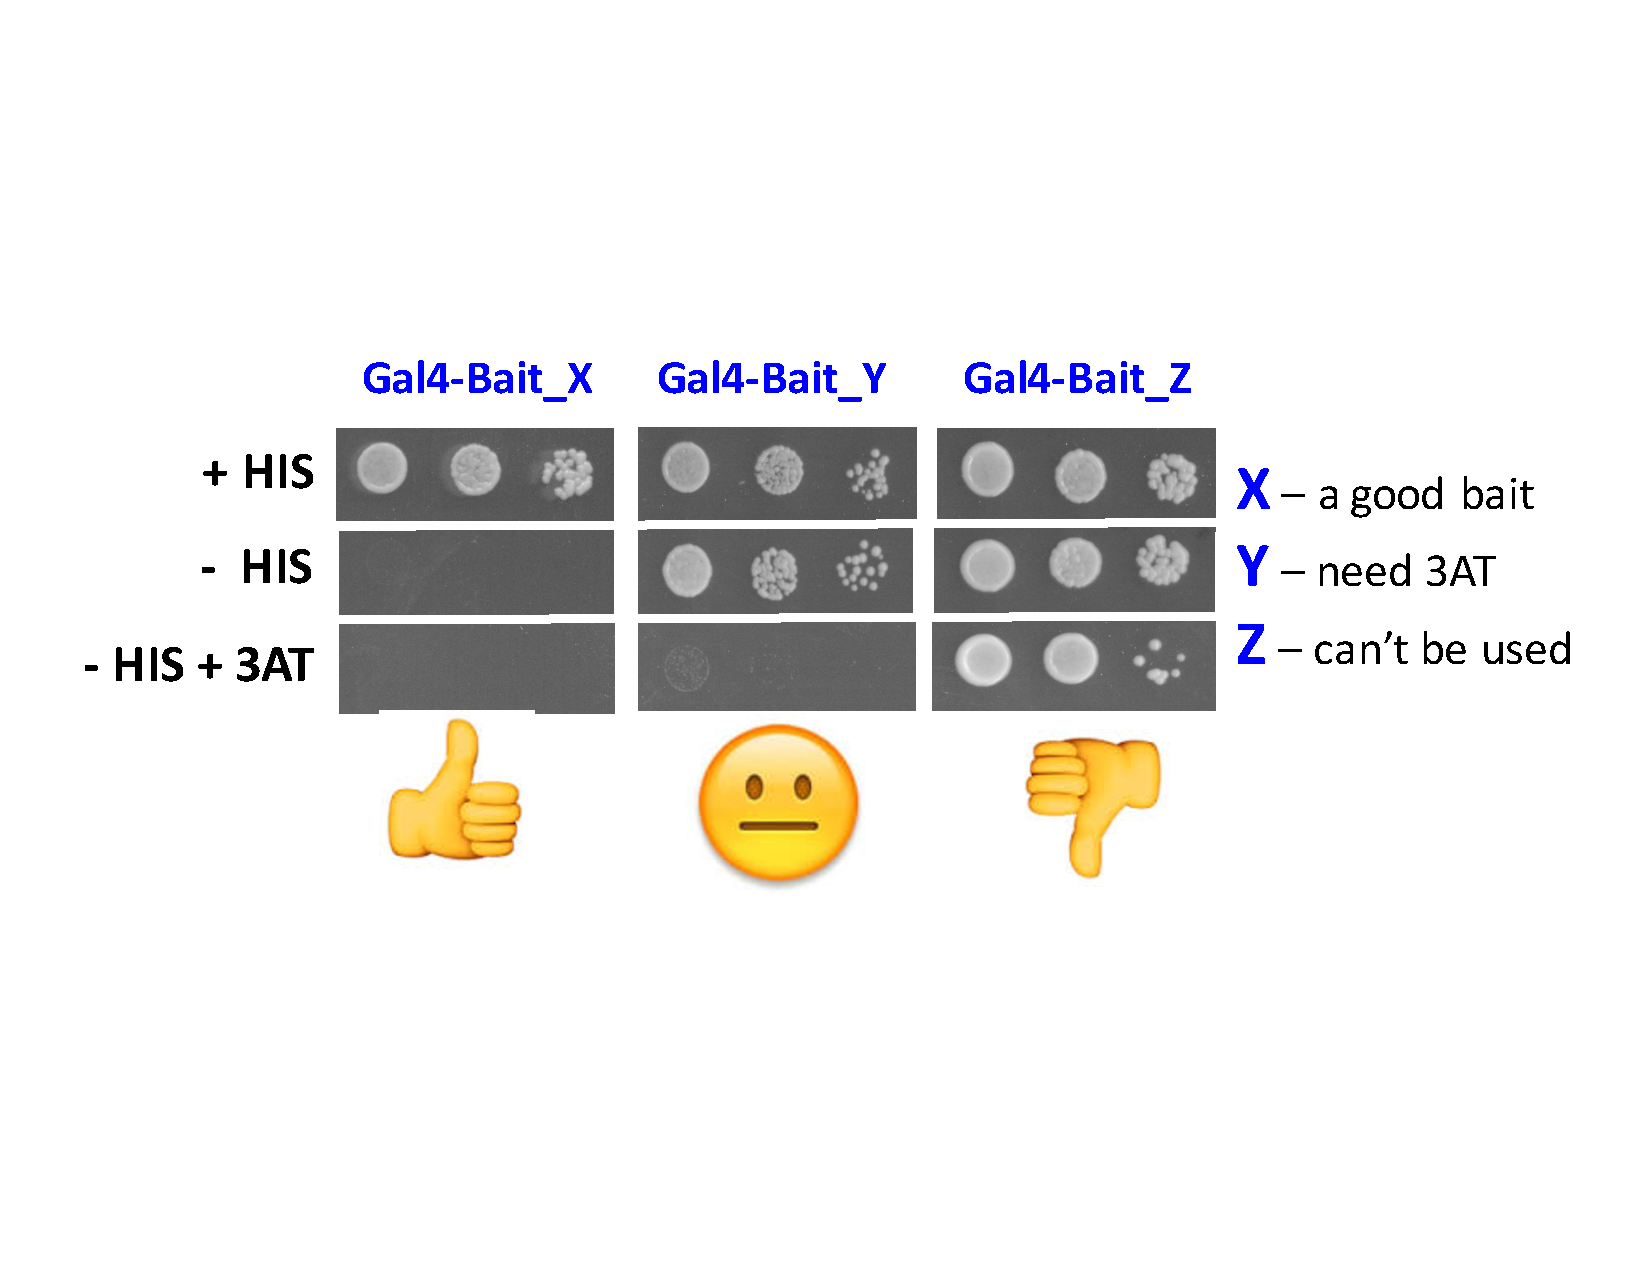
\includegraphics[width=\textwidth]{Exp1}
    \caption{}
    \label{fig:exp_fig1}
\end{figure}


\begin{remark}
    The best result is to see growth in the presence but not absence of Histidine regardless of whether there is 3AT.  This will allow the use of SD-Trp-Leu-His to select for yeast with a positive Y2H interaction.  If there is growth on SD-Leu-Trp-His plates, then a Y2H selection can still be obtained using the lowest concentration of 3AT that prevents growth.  Typically, the level of 3AT to establish a threshold of selection is between 0.1 and 1 mM.  This can be observed in Figure 1. Using higher levels of 3AT or other selections that are more stringent will undermine the ability to detect Y2H interactors.  If growth is observed on SD-Leu-Trp-His > 1mM 3AT a different bait plasmid should be sought.
\end{remark}

\subsection{Mating and Selection}

\begin{figure}[!ht]
    \centering
    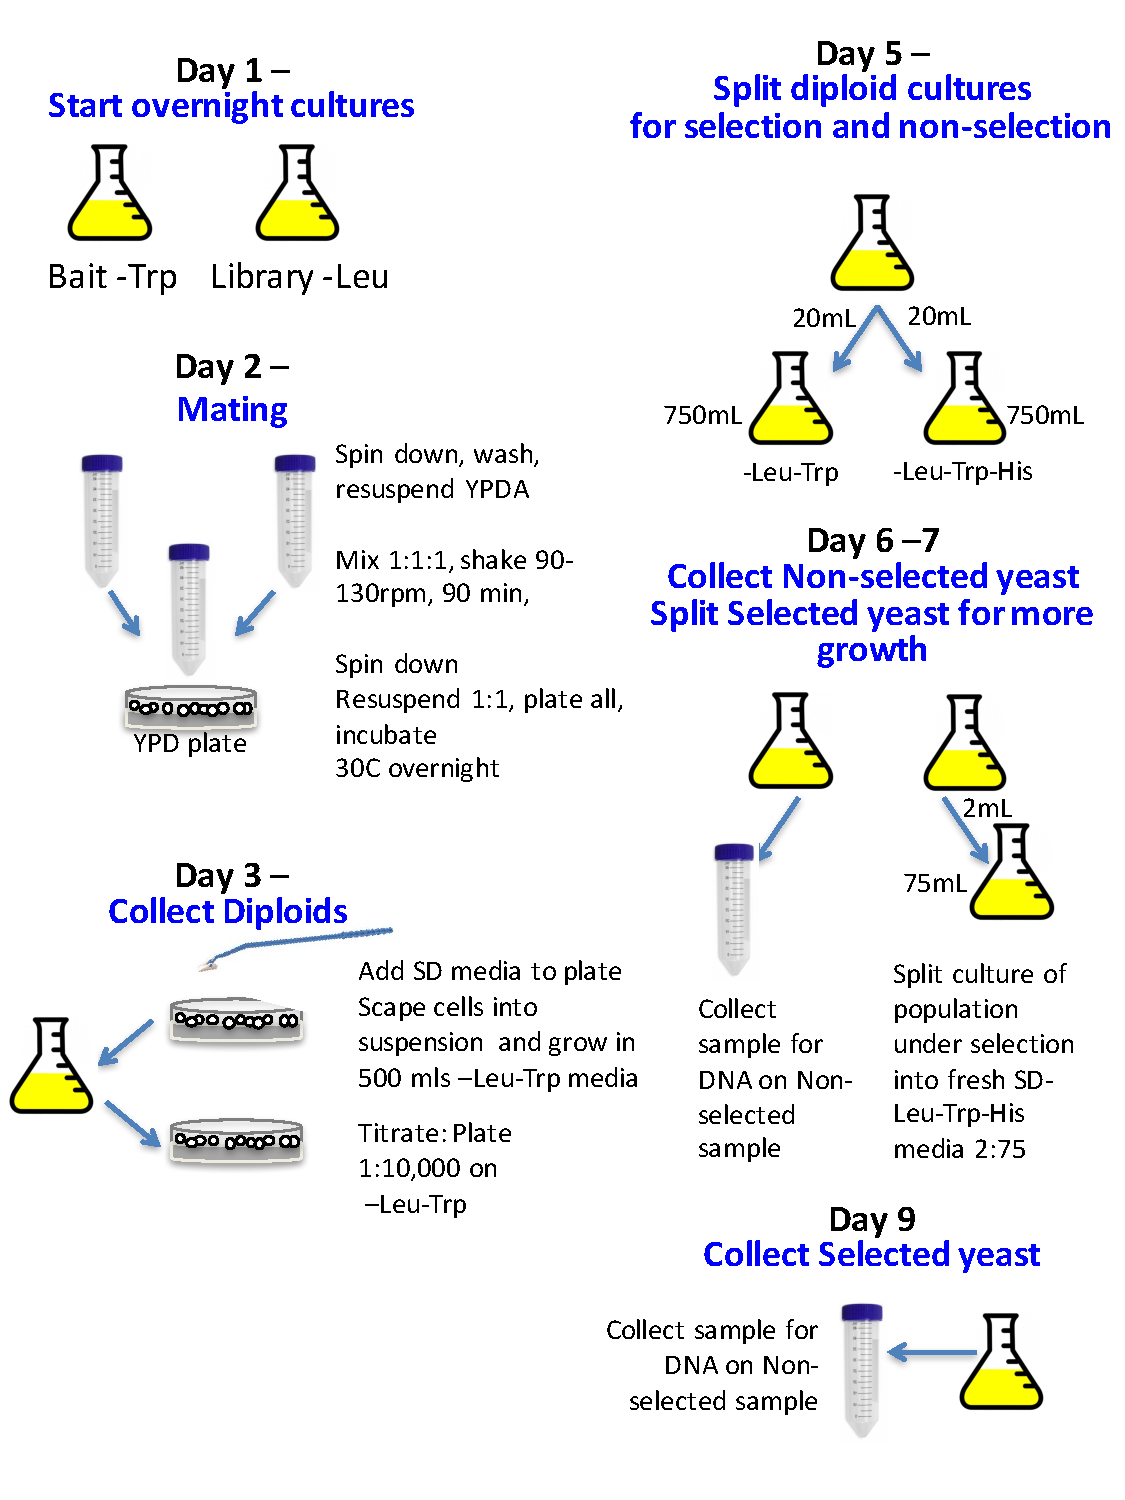
\includegraphics[width=\textwidth]{Exp2}
    \caption{}
    \label{fig:exp_fig2}
\end{figure}

The Y187 strain does not mate well.  Thus, the following optimized conditions are required to maintain complexity of the library.  The overall scheme is pictured in Figure 2.
\vspace{0.1in}
\begin{enumerate}[leftmargin=0.8in]
    \item[\textbf{Day 1}] Innoculate a fresh culture of the PJ69-4A strain transformed with the TRP1-containing bait plasmid in 23 mls of SD-Trp media. Thaw a vial of the Y187 cells containing the \emph{LEU2}-carrying “prey” library plasmid and inoculate a 125mls of SD-Leu media. Grow all cultures overnight at 30$^\circ$C, 200rpm.
    \item[\textbf{Day 2}] The O.D. of the overnight cultures should range between 1.0 to 1.5.  Pellet 21 OD equivalents of the PJ69-4A transformant cells and 15 OD equivalents of the Y187 strain carrying the library plasmids in separate 50mL conical tubes. Resuspend cells in 10ml of water and re-pellet in new 50 ml conical tube.  Resuspend PJ69-4A cells and Y187 cells in 4 ml bYPDA pH 3.7, each. To set-up 4 equivalent mating reactions, add 1mL PJ69-4A cells, 1ml Y187 cells, and 1 ml bYPDA pH 3.7 to new 50 ml conical tube. Incubate at 30$^\circ$C with gentle orbital agitation (90-130rpm) for 90 min so that the cells do not fully sediment.  Pellet cells, and resuspend in 2mls of bYPDA (See Appendix A). Plate all 2 mLs onto a 150 mm YPD plate.  
    \item[\textbf{Day 3}] Harvest cells from the YPD plates using 12 mls of SD-Leu-Trp media and place into a 50mL conical tube.  Pellet cells and resuspend the cells in 40 mLs SD-Leu-Trp media. To calculate the the number of diploid cells, dilute 4µls of the diploid mixture into 200 $\mu$ls SD-Trp-Leu media and plate onto an SD-Leu-Trp plate.  This plate represents a 1:10,000 fold dilution of the stock of diploids harvested and should yield 100-1000 colonies after plate is incubated at 30$^\circ$C for 2 days. 
    
    Take the remainder of each 40ml cell resuspension and inoculate a flask containing 500mls of SD-Leu-Trp media. Shake incubate these flasks at 30°C, 200rpm until they reach saturation (~2.0 OD/ml).  This typically takes about 36 hours.  
\end{enumerate}

\begin{remark}
    To harvest cells efficienctly from YPD agar plates, scrap the cells off the YPD plates using a cell scrapper and SD-Leu-Trp media into a 50mL conical tube.  This will take about 4 or 5 times of rinsing the YPD plate with 2 -3mls of SD-Leu-Trp media at a time. 
\end{remark}

\begin{enumerate}[leftmargin=0.8in]
    \item[\textbf{Day 4}] Monitor the growth of all flasks by checking the Optical Density.
    \item[\textbf{Day 5}] At this point, the titer plates should be ready to analyze, allowing verification of sufficient mating efficiency to maintain library complexity.  A minimum of 1 million total diploids is recommended for this workflow. Take 20 mls from the saturated 500 ml culture and use to inoculate flasks containing 750 mls SD-Leu-Trp media and another 20 mls to inoculate a flask containing 750 mls SD-Leu-Trp-His with the lowest level of 3AT that eliminates background growth in SD–His media. Mix the new cultures (770 mls) well and take an initial OD600.  Shake incubate cultures at 30$^\circ$C, 200rpm until reaching saturation, which typically occurs in ~24 hrs for the unselected SD-Leu-Trp culture and can take up to 40+ hrs for cultures under stringent selection for Y2H interactions.   
\end{enumerate}


\begin{warning}
    Make sure that you mix the 500mL flask well before taking 20mls out for inoculation because yeast can sediment quickly and cell suspension needs to be homogeneous. 
\end{warning}


\begin{enumerate}[leftmargin=0.8in]
    \item[\textbf{Day 6}] Once the unselected SD-Leu-Trp cultures have reached saturation (OD 2.0), remove 10 mls, pellet cells, and freeze at -20$^\circ$C or continue onto DNA extraction.  For the unselected SD-Leu-Trp culture, this will serve as the sample for sequencing.  
    \item[\textbf{Day 7}] Once the selected SD-Leu-Trp-His culture that is selecting for positive Y2H interactions has reached saturation, remove 2 mls of the culture and inoculate into 75 mls of fresh SD-Leu-Trp-His containing appropriate levels of 3AT. Allow this culture to grow at 30$^\circ$C with shaking at 200rpm until it reaches saturation, which can be followed throughout the course of growth by taking OD measurements. Saturation is typically attained within 30-60 hrs of growth.  
    \item[\textbf{Day 8-9}] Once the Selected SD-Leu-Trp-His cultures reach saturation (OD 2.0), remove 10 mls, pellet cells, and at this point cells can be frozen at -20$^\circ$C or continue onto the next step of DNA extraction.    
\end{enumerate}


\subsection{Sample preparation for DEEPN Illumina Sequencing}

\begin{enumerate}[leftmargin=1.4in]
    \item[\textbf{DNA Extraction}] Resuspend pellets of cells in 500ul of 50mMTris 20mMEDTA and transfer to a 1.5mL eppendorf tube. Add 3 $\mu$l of BME and 10 $\mu$l of Zymolase stock.  Mix well and incubate in the 37°C incubator for 24-36hours.  Extract with Phenol/Chloroform/Isoamyl alcohol and ethanol precipitate.  Resuspend pellet in 100 $\mu$l of 50mMTris/20mMEDTA add 1 $\mu$l of RNaseA stock and incubate at 37$^\circ$C for 1hr. Ethanol precipitate and resuspend in 100 $\mu$l 5mMTris/2mMEDTA.  Quantify DNA by absorbance at 280 nm.  
    \item[\textbf{2 PCR cDNA inserts}] Perform 2, 50$\mu$l PCR reactions per DNA sample.  Each reaction contains 50 pmoles F1-primer and R1-primer (Figure 3), 25µls NEBNext High-Fidelity 2x PCR Master Mix, 5 $\mu$g of DNA sample, and water up to 50 $\mu$l. The reactions are amplified for 25 cycles with extension times of 3 min. Analyze PCR products by agarose gel electrophoresis.  Samples should show smear of DNA around 1-3 kb, where the banding pattern may be found for samples where a yeast two-hybrid interaction was selected for (Figure 3).  Combine duplicate PCR samples and purify using the QIAquick PCR purification kit.  
    \item[\textbf{Illumina sequencing}] 550ng of PCR product was sheared using a Covaris E220 to give fragments of an average length of 300bp. Indexed Sequencing libraries were generated using the KAPA Hyper Prep kit Cat No: KK8500 (KAPA Biosystems, Wilmington, MA) for Illumina sequencing that adds linkers encoding barcodes, priming sites and capture sequences asymmetrically on the ends of the DNA fragments. Indexed libraries were then pooled and sequenced using the Illumina 2x100 nt SBS v3 chemistry run on an Illumina HiSeq2500 (Illumina, Inc., San Diego, CA). The number of reads targeted was between 10 and 30 million, with more reads desired for the unselected populations that are typically more complex.
\end{enumerate}

\begin{figure}[!ht]
    \centering
    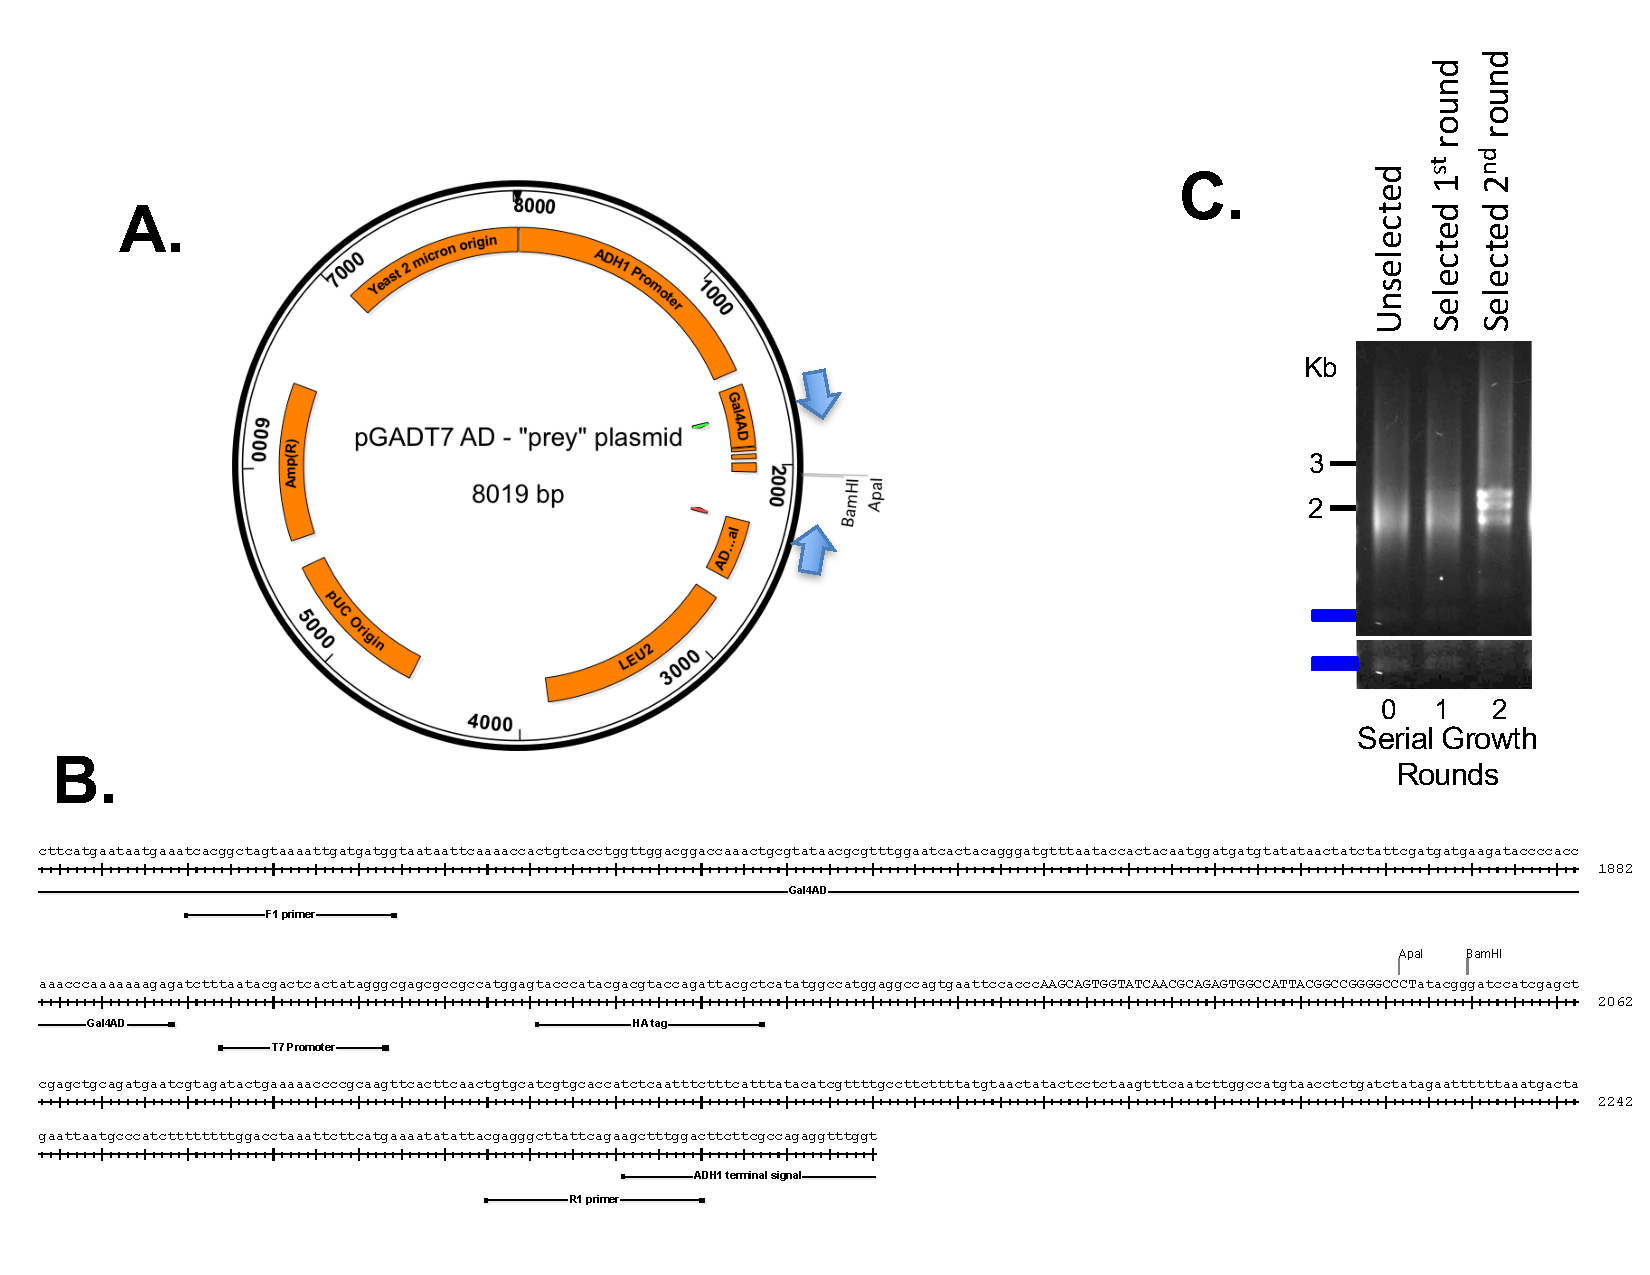
\includegraphics[width=\textwidth]{Exp3}
    \caption{}
    \label{fig:exp_fig3}
\end{figure}

%----------------------------------------------------------------------------------------
%	PART
%----------------------------------------------------------------------------------------

\part{Software}

%----------------------------------------------------------------------------------------
%	CHAPTER 1
%----------------------------------------------------------------------------------------

\chapterimage{chapter_head_1.pdf} % Chapter heading image

\chapter{DEEPN Software Overview}

\section{About DEEPN}\index{About DEEPN}
This user guide describes use of the standalone \DEEPN application and how to operate the modules within it.

The \DEEPN bioinformatics workflow is a collection of 4 programs

% \begin{wrapfigure}{l}{0.25\textwidth}
% 	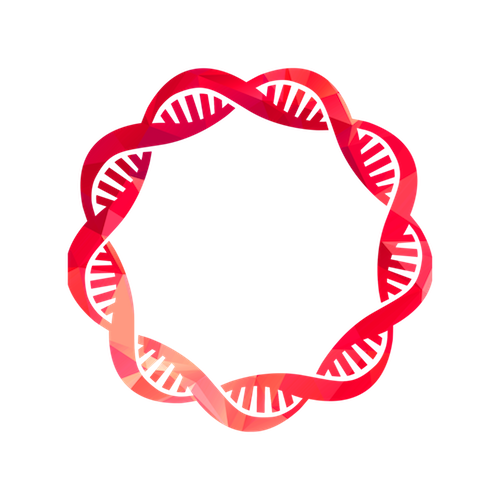
\includegraphics[width=0.9\linewidth]{Pictures/gene_count.png} 
% 	\caption{Caption1}
% 	\label{fig:subim1}
% 	\end{wrapfigure}
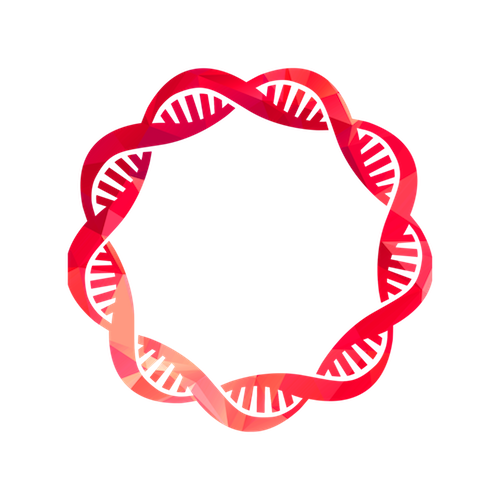
\includegraphics[scale=0.3]{Pictures/gene_count.png} \GeneCount counts the number of sequence reads found for every gene.\\

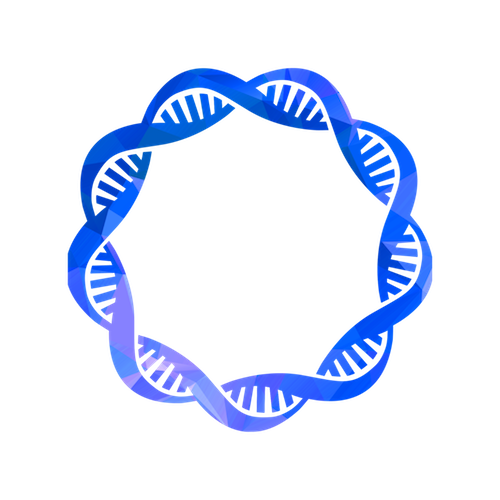
\includegraphics[scale=0.3]{Pictures/junction_make.png} \JunctionMake finds and identifies all the sequences corresponding to the junction sequences that span the end of the bait plasmid with the cDNA insert in the library “prey” plasmid.\\

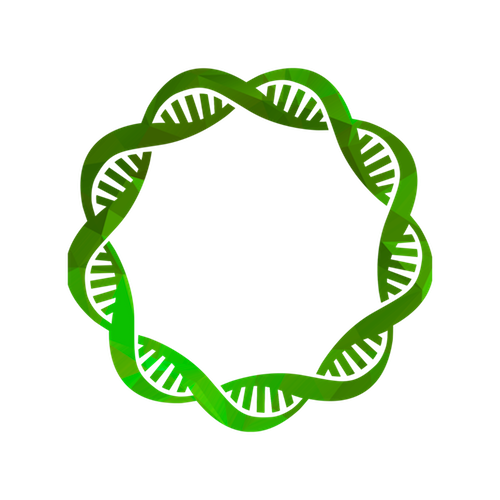
\includegraphics[scale=0.3]{Pictures/query_blast.png} \BlastQuery allows the junction sequences to be analyzed.\\

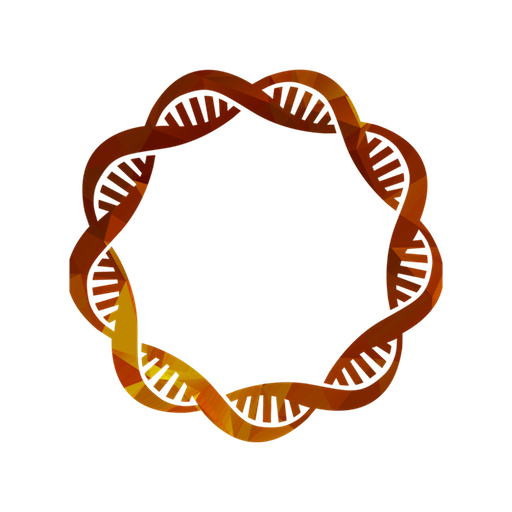
\includegraphics[scale=0.3]{Pictures/read_depth.png} \ReadDepth calculates the read depth for a particular cDNA, useful for \\predicting the 3’ end of a cDNA insert.

\vspace{15pt}

\DEEPN was developed to process and analyze sequence information from the Illumina platform that produces 110-140 bp reads.  Both single and paried-end sequences are appropriate, \DEEPN considers the different sides of a paried-end sequence as two separate sequences. \DEEPN requires sequence files in \texttt{.sam} format, in which sequences have been mapped to the genome.  Processing of .fastq sequence files with \texttt{Tophat2} will work, producing unmapped and mapped \texttt{.sam} files for each fastq read file. \DEEPN requires BOTH mapped and unmapped \texttt{.sam} files to fully analyze a sequence dataset. See Section \ref{download link} for download link.

    Samtools (http://goo.gl/Uhr10S), Tophat2 (https://goo.gl/16BNHo), and Bowtie2 (http://goo.gl/NwVXZ) need to be used for mapping the reads.

    \DEEPN considers each sequence read separately. Thus, if Paired-End reads were collected, they need not be mapped as such by Tophat2 or Bowtie2.  \DEEPN does not care.  Thus, for Paried End reads that give two sample files (eg. Sample\_R1.fastq and Sample\_R2.fastq) it is easier to concantnate both the *\_R1 and *\_R2 files together and then map the merged file data as a Single End reads.

    Example:

      cat Sample\_R1.fastq Sample\_R2.fastq >> CombinedSample.fastq  
                 (concatenates files)

      ./tophat2 -o TophatOutput/ -p 11 ./indexes/mm10 
                 (maps reads)

      samtools view -h -o CombinedSample.unmapped   ./TophatOutput/unmapped.bam 
                 (converts .bam file of unmapped reads to .sam file)

      samtools view -h -o CombinedSample.mapped   ./TophatOutput/accepted\_hits.bam 
                 (converts .bam file of mapped reads to .sam file)


\begin{remark}
	Later releases of DEEPN for Mac will also contain functions to automatically map \texttt{.fastq} files with Tophat2 to allow for seamless integration of processing sequence data.\\

	\texttt{.fastq} $\,\to\,$ Tophat2/Bowtie $\,\to\,$ \GeneCount $\,\to\,$ {\color{Blue} Junction Make} $\,\to\,$ {\color{ForestGreen} Blast Query} $\,\to\,$  {\color{Bittersweet} Read Depth}.  
\end{remark}


The \DEEPN application provides a graphic user interface to guide the launch and operation of \GeneCount, \JunctionMake, \BlastQuery, or \ReadDepth modules within it. \DEEPN comes in versions that run on Windows and Mac operating systems. See Section \ref{download link} for download link.

\clearpage



\section{Contents within DEEPN}\index{Contents within DEEPN}

\begin{enumerate}
\item Program modules
	\begin{itemize} 
		\item {\color{Red} Gene Count}
		\item {\color{Blue} Junction Make}
		\item {\color{ForestGreen} Blast Query}
		\item {\color{Bittersweet} Read Depth}
	\end{itemize}
which are launched from within the main DEEPN.app or DEEPN.exe.
\item Databases for the Gene and mRNA coordinates
	\begin{itemize} 
		\item mouse mm10 genome and mouse RefSeq data
		\item Gene and ORF coordinates for the SacCer3 genome
	\end{itemize}
These allow analysis of mouse cDNA Y2H libraries and yeast genomic Y2H libraries.  The modified mouse and human RefSeq database that \DEEPN uses contains just the known annotated mRNAs, basically the entries that have an \texttt{NM\_*} nomenclature in genbank.  It does not contain microRNAs, long non-coding RNAs, and theoretical splice variants. \DEEPN contains a database of yeast genes, with a hybrid nomenclature of their systematic SGD name and their genebank \texttt{NM\_*} nomenclature.  For simplicity, a given yeast gene consists of the protein coding sequence flanked by 100 bp of untranslated region.
	
\item Database of ``junction tags'' for different libraries.  Currently, analysis of the mouse cDNA libraries defaults to the use of the Clontech mate/plate pGADT7 plasmid and uses the GRCm38/mm10. This is also the case for analysis of human cDNA library that uses the GRCh38/hg38 reference genome data  And analysis of the yeast libraries is tied to the Phil James libraries housed in pGAD-C1, C2, and C3 \emph{(James et al., 1996)}. The yeast Y2H library analysis uses the sacCer3(April 2011) database. These default junction tags from these libraries are:
	\begin{itemize} 
		\item cDNA insert (mouse and human)
		\begin{lstlisting}
		AATTCCACCCAAGCAGTGGTATCAACGCAGAGTGGCCATTACGGCCGGGG
		\end{lstlisting}
		\item genomic fragment insert (\emph{S. cerevisiae})
		\begin{lstlisting}
		ATGATGAAGATACCCCACCAAACCCAAAAAAAGAGATCGAATTCCCGGGG
		\end{lstlisting}
	\end{itemize}
	\begin{remark} 
		Users can insert their own junction sequence into the \DEEPN dialog box if using a different library.  For a more permanent solution, users can modify the SQL database that houses these data (see below)
	\end{remark}
\item \DEEPN operates the \texttt{blastn} program while its processing data.  That is called upon by the \JunctionMake program.  All of the relevant files required to blast search mouse mRNAs or yeast genes are included in internal resources.  Stand-alone Blastn program and associated databases to perform \texttt{blastn} locally from within the \DEEPN application.
\end{enumerate}


\section{DEEPN WorkFlow Overview}\index{DEEPN Workflow Overview}

\begin{center}
	\smartdiagram[descriptive diagram]{
		{Select \textbf{Work Folder}, Locate a folder in your computer where you like the analysis to be performed.},
		{Place \texttt{.sam} files, Place .sam files within the \textbf{mapped\_sam\_files} and \textbf{unmapped\_sam\_files} subfolders within the selected \textbf{Work Folder}.},
		{Process Data, Use \GeneCount and \JunctionMake to process data. This will create several subfolders containing the processed data},
		{Analyze Data, {Using \BlastQuery and \ReadDepth}},
	}
\end{center}
Step-by-step screen-shots and instructions are detailed in the following chapters.


%------------------------------------------------

\section{Installation}\index{Installation}
\subsection{Download Link}\label{download link}\index{Download Link}

    Platform-specific compiled binaries (\emph{Mac OS X, Windows and Linux}) of \textbf{DEEPN} can be downloaded from the below URL. \\

    \texttt{\href{https://github.com/emptyewer/DEEPN/releases}{https://github.com/emptyewer/DEEPN/releases}}

    \subsection{Mac OS X Compatibility}\index{Mac OS X Compatibility}\label{mac_install}

    \texttt{Mac OS X (10.10+) Yosemite and above}

    \subsection{Windows Compatibility}\index{Windows Compatibility}\label{windows_install}

    \texttt{64-bit or 32 bit Windows 7 and above. Note that \DEEPN itself is a 32-bit software.}

    \subsection{Linux Compatibility}\index{Linux Compatibility}\label{linux_install}

    \texttt{Scheduled for release in Version 2.0 of DEEPN.}

\clearpage

\section{Open Source License}\index{Open Source License}\label{license}
\begin{lstlisting}

The MIT License (MIT)

Copyright (c) 2016 Venkatramanan Krishnamani, Robert C. Piper, Mark Stammnes

Permission is hereby granted, free of charge, to any person obtaining a copy
of this software and associated documentation files (the "Software"), to deal
in the Software without restriction, including without limitation the rights
to use, copy, modify, merge, publish, distribute, sublicense, and/or sell
copies of the Software, and to permit persons to whom the Software is
furnished to do so, subject to the following conditions:

The above copyright notice and this permission notice shall be included in all
copies or substantial portions of the Software.

THE SOFTWARE IS PROVIDED "AS IS", WITHOUT WARRANTY OF ANY KIND, EXPRESS OR
IMPLIED, INCLUDING BUT NOT LIMITED TO THE WARRANTIES OF MERCHANTABILITY,
FITNESS FOR A PARTICULAR PURPOSE AND NONINFRINGEMENT. IN NO EVENT SHALL THE
AUTHORS OR COPYRIGHT HOLDERS BE LIABLE FOR ANY CLAIM, DAMAGES OR OTHER
LIABILITY, WHETHER IN AN ACTION OF CONTRACT, TORT OR OTHERWISE, ARISING FROM,
OUT OF OR IN CONNECTION WITH THE SOFTWARE OR THE USE OR OTHER DEALINGS IN THE
SOFTWARE.
\end{lstlisting}


\chapter{Initial Setup}

\section{Preprocessing \texttt{.fastq files}}\index{Preprocessing \texttt{.fastq files}}

The current DEEPN application requires that \texttt{.sam} files have been generated from the \texttt{.fastq} Illumina sequence files.  This is done using the mapping program \texttt{Tophat2}, which itself runs on top of \texttt{Bowtie}.  It is imperative that downstream processing by DEEPN uses the same databases that \texttt{Tophat2} uses to map the sequence files. These are...

\begin{enumerate}
	\item Mouse: mm10\/GRCm38 2011 \emph{Mus musculus} assembly (Genome Reference Consortium Mouse Build 38 (\texttt{GCA\_000001635.2})\\
	\texttt{\href{https://goo.gl/T6OT2F}{https://goo.gl/T6OT2F}}
  \item Human: hg38\/GRCh38 2013 \emph{Mus musculus} assembly (Genome Reference Consortium Human Build 38 (\texttt{GCA\_000001405.15})\\
  \texttt{\href{https://goo.gl/xWgczW}{https://goo.gl/xWgczW}}
	\item Yeast: sacCer3 2011 \emph{Saccharomyces cerevisiae} S288c assembly from Saccharomyces Genome Database (\texttt{GCA\_000146055.2})\\
	\texttt{\href{https://goo.gl/wfPbvA}{https://goo.gl/wfPbvA}}
\end{enumerate}

\texttt{Tophat2} should produce sets of .sam files of Mapped Reads and Unmapped Reads for every input .fastq file.  DEEPN will use both of these files.

\section{Initializing DEEPN}\index{Initializing DEEPN}

\subsection{Launching}\index{Launching DEEPN}
Open the \DEEPN application by double clicking. This opens a window (DEEPN) that can be used to run the other modules.
\begin{itemize}
	\item[\textbf{Step 1.}] \textbf{Select Parameters from the list menu in the top. Figure \ref{fig:deepn_main_window}}
	\begin{itemize}
		\item Selecting the \emph{M. musculus} option selects the mm10 mouse databases
    \item Selecting the Human option selects the hg38 Human databases
		\item Selecting the \emph{S. cerevisiae} option selects the sacCer3 yeast databases
		\item Once this is selected, the “Select Work Folder” will be activated for use
	\end{itemize}
	\begin{figure}[!ht]
	    \centering
	    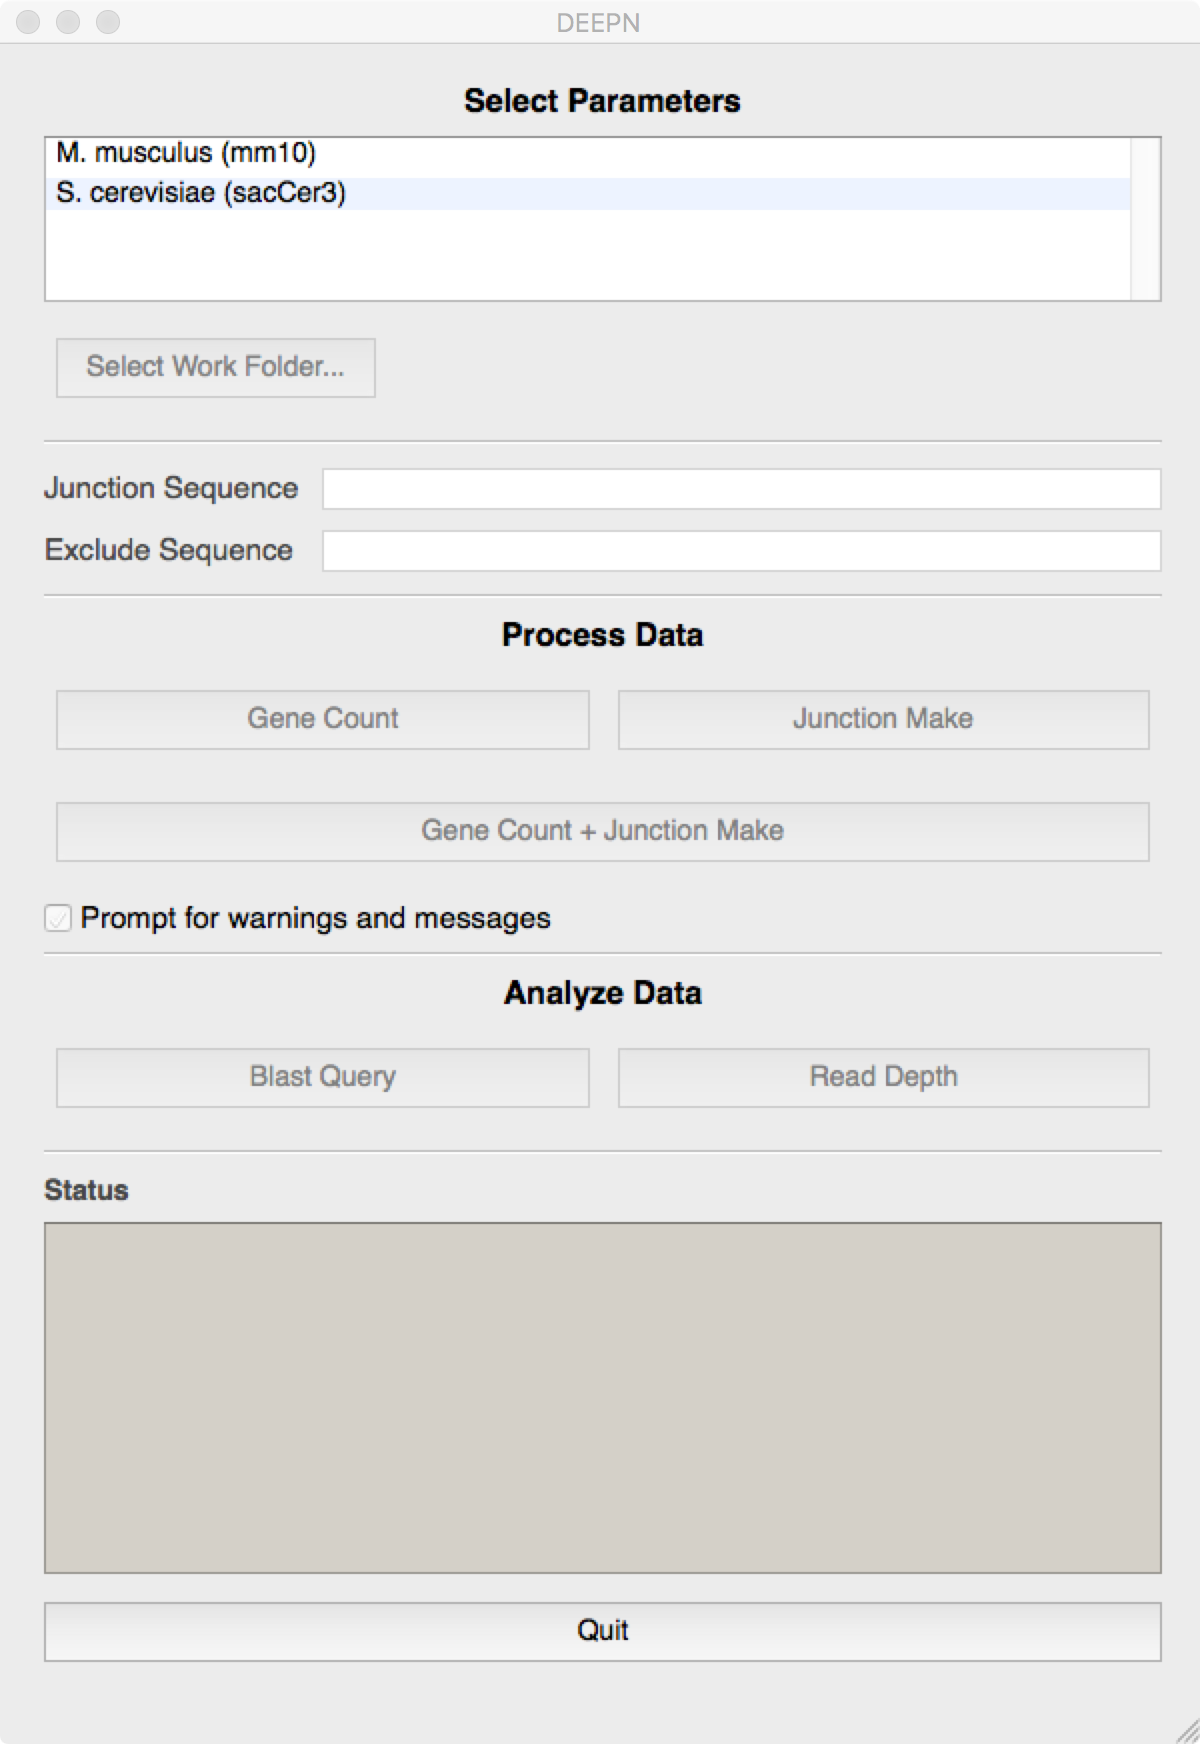
\includegraphics[width=0.8\textwidth]{figure1}
	    \caption{\DEEPN main interface.}
	    \label{fig:deepn_main_window}
    \end{figure}
	\item[\textbf{Step 2.}] \textbf{Create a work folder Figure \ref{fig:select_work_folder}}

	\begin{itemize}
		\item \DEEPN needs a folder to write its files into and to read sequence files from.  This is done using the ``Select Work Folder'' button 
\includegraphics[width=80pt]{Pictures/work_folder_btn}. Here create a new folder or select an existing one.
		\item Once your Work Folder is designated, \DEEPN will need to operate from two subfolders within it (See Figure \ref{fig:select_work_folder}). These folders are called...
		\begin{itemize}
			\item \texttt{mapped\_sam\_files}
			\item \texttt{unmapped\_sam\_files} 
		\end{itemize}
		\item If these folders already exist within the ``Work Folder'' because of previous processing, then \DEEPN will use them.
		\item If the ``Work Folder'' is new and those folders do not exist, \DEEPN will create them.
	\end{itemize}
	\begin{figure}[!ht]
	    \centering
	    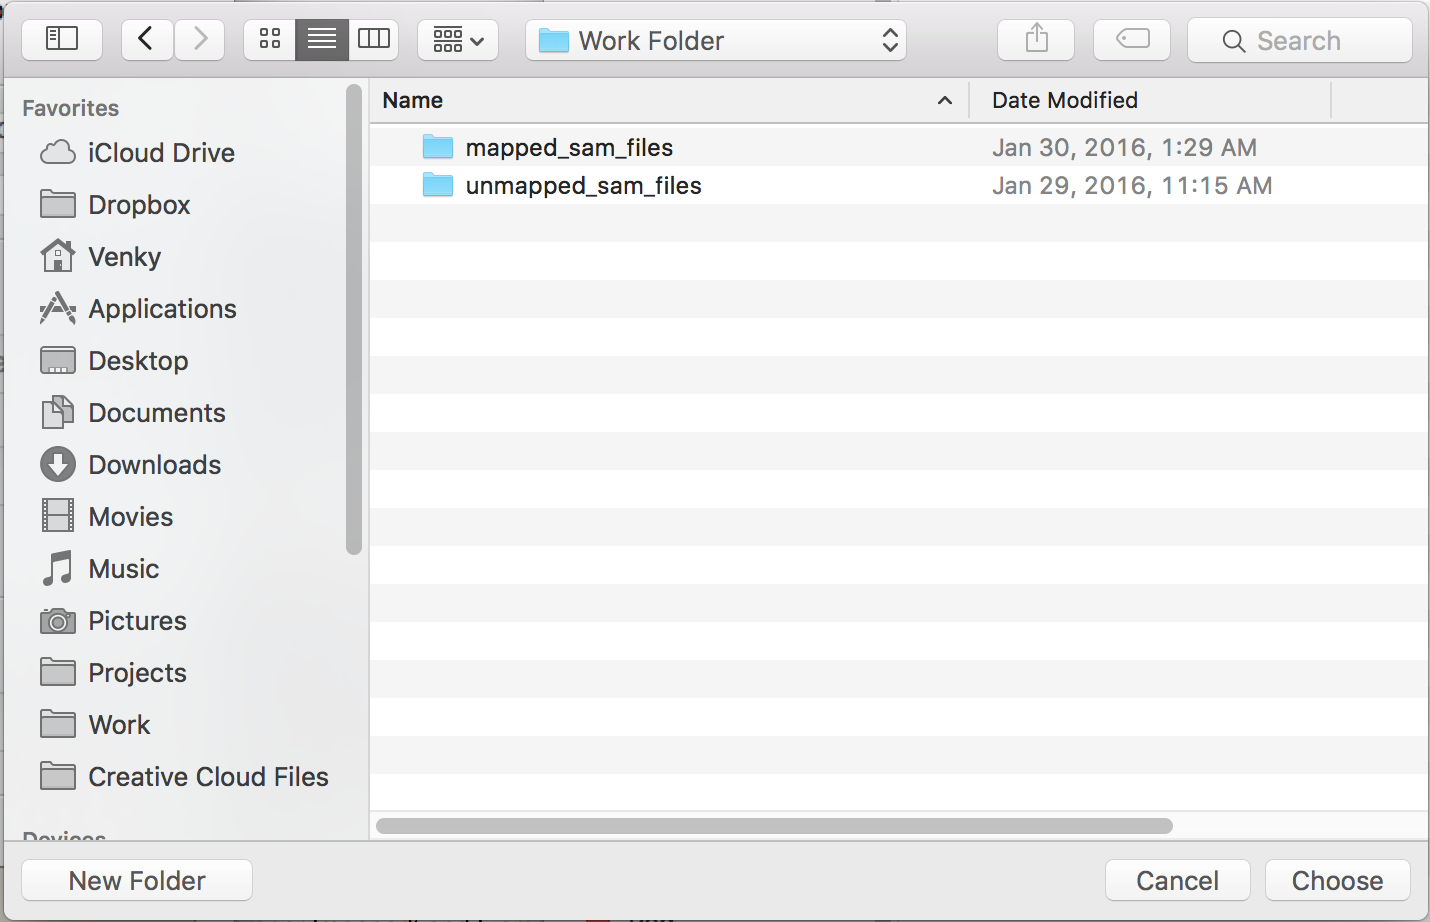
\includegraphics[width=0.8\textwidth]{work_folder}
	    \caption{Folder with two subfolders, named \texttt{mapped\_sam\_files} and \texttt{unmapped\_sam\_files} is the starting state of \DEEPN work folder before processing.}
	    \label{fig:select_work_folder}
    \end{figure}

    \item[\textbf{Step 3.}] To start things off, move your \texttt{.sam} files generated by \underline{Tophat2} into the \texttt{mapped\_sam\_files} and \texttt{unmapped\_sam\_files} folders.
\end{itemize}

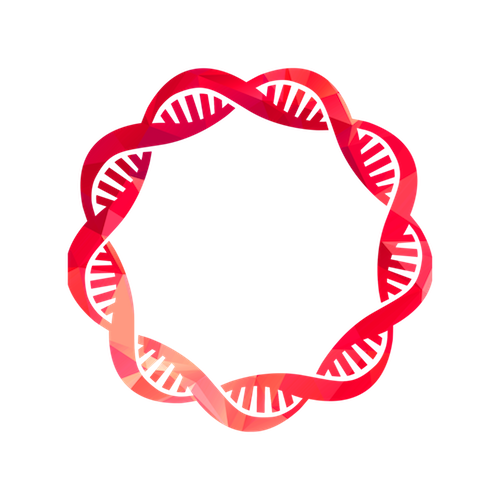
\includegraphics[scale=0.3]{Pictures/gene_count.png} \GeneCount module will process the \texttt{.sam} files placed in the \texttt{mapped\_sam\_files} folder. These files should contain the mapped read files outputted from \underline{Tophat2}\\

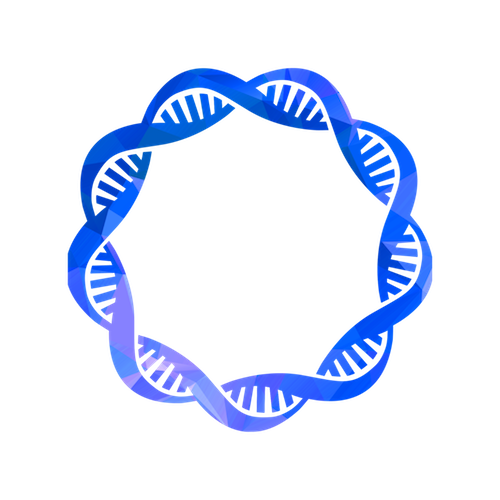
\includegraphics[scale=0.3]{Pictures/junction_make.png} \JunctionMake module will process the \texttt{.sam} files placed in the \texttt{unmapped\_sam\_files} folder. These files should contain the \underline{UNmapped} read files outputted from \underline{Tophat2}.  These are the reads that were unable to to mapped adequately to the \textbf{SacCer3} or the \textbf{Mm10} genomes and that contains the bulk of junction reads. With Illumina 110-120 bp reads, the stretch of cDNA or gene DNA in these ``Junction sequences'' is too short to be mapped to a chromosome by \underline{Tophat2}. This workflow assumes these types of short reads.  Were one to have longer reads, the Junction Sequences might be able to be mapped, which would oblige the search for them to included the Mapped reads as well.\\

\begin{itemize}
	\item Once \texttt{.sam} files are placed within \texttt{mapped\_sam\_files}, the 
\includegraphics[width=120pt]{Pictures/gene_count_btn} button is activated and the \GeneCount processing can begin by clicking the button.
	\item Once \texttt{.sam} files are placed within \texttt{unmapped\_sam\_files}, the 
\includegraphics[width=120pt]{Pictures/junction_make_btn} button is activated and the \JunctionMake processing can begin by clicking the button.
\end{itemize}

\begin{warning}
A warning message may appear if \DEEPN detects folders created by previous processing runs. \DEEPN will add to these folders, but users run the risk that if file names are the same, the old files will be written over by the new files. To avoid any problems, one can move the processed data folders to a new location.
\end{warning}

%----------------------------------------------------------------------------------------
%	PART
%----------------------------------------------------------------------------------------

\part{Processing Data}

%----------------------------------------------------------------------------------------
%	CHAPTER 3
%----------------------------------------------------------------------------------------

\chapterimage{chapter_head_1.pdf} % Chapter heading image

\chapter{\GeneCount}\index{Gene Count}

\GeneCount will process all the \texttt{.sam} files that are in the folder \texttt{mapped\_sam\_files}

\vspace{15pt}

Once the \texttt{.sam} files are moved to this folder, click the 
\includegraphics[width=120pt]{Pictures/gene_count_btn} button.

\begin{remark}
Clicking the 
\includegraphics[width=120pt]{Pictures/gene_count_btn} button will only be possible if there are files in \texttt{mapped\_sam\_files} folder.
\end{remark}

After starting, \GeneCount will report to you the following:

\begin{lstlisting}
>>>GENEcountY2H
Gene Count will process the mapped .sam files present in the folder mapped_sam_files
Gene Count will generate two folders for its output data:
gene_count_summary contains a summary files of genes and their count frequency. 
chromosome_files contains more granular data for each gene.

Be patient....This program is slow but will keep you posted.
>>>END
\end{lstlisting}

\GeneCount will populate the \texttt{gene\_count\_summary} and \texttt{chromosome\_files} folders with files that have names corresponding to the input files. 

For an input file named \textbf{\texttt{Dataset1.sam}}
\begin{itemize}
	\item The \texttt{gene\_count\_summary} folder will contain \textbf{\texttt{Dataset1\_summary.csv}}
	\item The \texttt{chromosome\_files} folder will contain \textbf{\texttt{Dataset1\_ChrGene.csv}}
\end{itemize}

\vspace{15pt}
The \texttt{\_summary.csv} files generated by \GeneCount have the following format when opened in \texttt{Microsoft Excel}. See Figure \ref{fig:excel_screen_shot}.

\begin{itemize}
	\item The name of the \texttt{.sam} file processed is found along the top.
	\item \textbf{Column A} shows Chromosome on which each gene is located
	\item \textbf{Column B} shows gene name
	\item \textbf{Column C} shows the frequency of reads for that gene in parts per million (PPM)
	\item \textbf{Columns D and greater} show corresponding NCBI genbank accession numbers that describe annotated mRNA sequences for that gene
\end{itemize}

Shown are the ``TotalReads'' that were found in the starting \texttt{.sam} file (Total Mapped Reads). Also shown are the ``TotalReads(PPM)'' that were used in the PPM calculation (TotalReads that were used in the PPM calculation).  TotalReads is often significantly larger than TotalReads(PPM) because many of the mapped reads cannot be assigned to a particular gene.  This is the case with the genomic libraries that have lots of fragments that do not encode exons.  It also is the case with cDNA libraries that have splice variants and other sequences that do not correspond to what is currently annotated as an exon for that corresponding gene.

\begin{remark}
TotalReads(PPM)) is the number of reads that were found to have a position corresponding to a known exon as annotated in the corresponding database used. Since some exons have yet to be annotated, some of the reads may not be able to be assigned to a particular gene, which accounts for the discrepancy between TotalReads(PPM) and TotalReads.
\end{remark}



\begin{figure}[!ht]
    \centering
    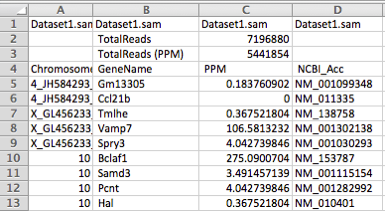
\includegraphics[width=0.8\textwidth]{excel}
    \caption{Screen-shot of \texttt{\_summary.csv} file generated by \GeneCount.}
    \label{fig:excel_screen_shot}
\end{figure}



\chapter{\JunctionMake}\index{Junction Make}

\JunctionMake will process all the \texttt{.sam} files that are in the folder \texttt{unmapped\_sam\_files}.

\vspace{15pt}

Once the \texttt{.sam} files are moved to this folder, click the 
\includegraphics[width=120pt]{Pictures/junction_make_btn} button.

\begin{remark}
Clicking the 
\includegraphics[width=120pt]{Pictures/junction_make_btn} button will only be possible if there are files in \texttt{unmapped\_sam\_files} folder.
\end{remark}


\JunctionMake will report to you the following:

\begin{lstlisting}
>>>Comment1
- Make sure all ".SAM" files from your UNmapped reads are in the folder:
unmapped_sam_files
- This program will scan for junction sequences that span the Gal4 activation domain and the prey.
- The junction tag sequence used will be the one entered in the Junction Sequence textbox
- Output files will be placed in the junction_files folder as .junctions.txt files. 
- Blast identified reads will be placed in the blast_results folder as .blast.txt files
- A database of identified junctions will be placed in the blast_results_query folder as .p files
>>>END
\end{lstlisting}



\JunctionMake  will make the \texttt{junction\_files}, \texttt{blast\_results}, and \texttt{blast\_results\_query} folders to accept the new files it will produce. If these folders already exist, a warning will be issued to alert the user that files might be overwritten if \JunctionMake is run again. To avoid this, move the files out of the \texttt{junction\_files}, \texttt{blast\_results}, and \texttt{blast\_results\_query} folders to a new place or Abort, rename the \texttt{junction\_files}, \texttt{blast\_results}, and \texttt{blast\_results\_query} folders and start \JunctionMake again.


\JunctionMake will look for different junction ``tag'' sequence. When different \texttt{Gal4AD-} libraries are used, here is where some user input may be necessary.

\vspace{15pt}

For the \textbf{clontech mate and plate library} the junction ``tag'' sequence looked for is:
\begin{lstlisting}
AATTCCACCCAAGCAGTGGTATCAACGCAGAGTGGCCATTACGGCCGGGG
\end{lstlisting}


So Junction Sequences look like this for the mouse cDNA Mate/Plate pGADT7 library (Figure \ref{fig:cdna-junction}):
%\begin{lstlisting}
%AATTCCACCCAAGCAGTGGTATCAACGCAGAGTGGCCATTACGGCCGGGG||tcg-gac-aac-gca
%\end{lstlisting}

\begin{figure}[!ht]
\centering
\begin{texshade}{cdna.aln}
	\residuesperline*{40}
%	\vblockspace{-0.1in}
	\charstretch{1.5}
	\linestretch{1.5}
%	\hidel‘egend
%	
	\nameseq{1}{}
	\nameseq{2}{}
	\shadingmode{functional}
	\hideconsensus
	\hidenumbering
	\shaderegion{1}{51..66}{Black}{LightYellow}
%	\shaderegion{1}{72..74}{White}{Red}
%	\shaderegion{2}{74..76}{White}{Red}
%	\tintblock{1}{73..74}
%	
%	\shaderegion{2}{1..7}{Black}{LightYellow}
%	\shaderegion{2}{66..72}{Black}{LightYellow}
%	\shaderegion{2}{10..13}{Black}{LightProcessBlue}
%	\shaderegion{2}{22..25}{Black}{LightProcessBlue}
%	\shaderegion{2}{27..31}{Black}{LightLimeGreen}
%	\shaderegion{2}{39..43}{Black}{LightLimeGreen}
%	\shaderegion{2}{49..53}{Black}{LightLavender}
%	\shaderegion{2}{61..65}{Black}{LightLavender}
%	
%	\shaderegion{1}{1..7}{Black}{LightYellow}
%	\shaderegion{1}{64..71}{Black}{LightYellow}
%	\shaderegion{1}{10..12}{Black}{LightProcessBlue}
%	\shaderegion{1}{22..24}{Black}{LightProcessBlue}
%	\shaderegion{1}{26..30}{Black}{LightLimeGreen}
%	\shaderegion{1}{38..42}{Black}{LightLimeGreen}
%	\shaderegion{1}{47..51}{Black}{LightLavender}
%	\shaderegion{1}{59..63}{Black}{LightLavender}
%	
	\feature{ttop}{1}{51..66}{---[Red]}{Downstream Reading Frame}
%	\feature{bbottom}{2}{74..76}{---[Red]}{}
	\feature{ttop}{1}{1..50}{---[RoyalBlue]}{Junction Sequence}
%	\feature{bbottom}{2}{34..36}{---[RoyalBlue]}{}
\end{texshade}
\caption{Junction Sequences look like this for the mouse cDNA Mate/Plate pGADT7 library}
\label{fig:cdna-junction}
\end{figure}


\vspace{15pt}

For the \textbf{yeast genomic Phil James (pGAD-C1,2,3) library} the junction ``tag'' sequence looked for is:
\begin{lstlisting}
ATGATGAAGATACCCCACCAAACCCAAAAAAAGAGATCGAATTCCCGGGG
\end{lstlisting}

So junction sequences look like this for the pGAD-C yeast genomic library (Figure \ref{fig:gene-junction}):
% \begin{lstlisting}
% ATACCCCACCAAACCCAAAAAAAGAGATCGAATTCCCCGGGGGATCCATC||ggc-gaa-aac-gaa
% \end{lstlisting}

\begin{figure}[!ht]
\centering
\begin{texshade}{gene.aln}
	\residuesperline*{40}
%	\vblockspace{-0.1in}
	\charstretch{1.5}
	\linestretch{1.5}
%	\hidel‘egend
%	
	\nameseq{1}{}
	\nameseq{2}{}
	\shadingmode{functional}
	\hideconsensus
	\hidenumbering
	\shaderegion{1}{51..66}{Black}{LightYellow}
%	\shaderegion{1}{72..74}{White}{Red}
%	\shaderegion{2}{74..76}{White}{Red}
%	\tintblock{1}{73..74}
%	
%	\shaderegion{2}{1..7}{Black}{LightYellow}
%	\shaderegion{2}{66..72}{Black}{LightYellow}
%	\shaderegion{2}{10..13}{Black}{LightProcessBlue}
%	\shaderegion{2}{22..25}{Black}{LightProcessBlue}
%	\shaderegion{2}{27..31}{Black}{LightLimeGreen}
%	\shaderegion{2}{39..43}{Black}{LightLimeGreen}
%	\shaderegion{2}{49..53}{Black}{LightLavender}
%	\shaderegion{2}{61..65}{Black}{LightLavender}
%	
%	\shaderegion{1}{1..7}{Black}{LightYellow}
%	\shaderegion{1}{64..71}{Black}{LightYellow}
%	\shaderegion{1}{10..12}{Black}{LightProcessBlue}
%	\shaderegion{1}{22..24}{Black}{LightProcessBlue}
%	\shaderegion{1}{26..30}{Black}{LightLimeGreen}
%	\shaderegion{1}{38..42}{Black}{LightLimeGreen}
%	\shaderegion{1}{47..51}{Black}{LightLavender}
%	\shaderegion{1}{59..63}{Black}{LightLavender}
%	
	\feature{ttop}{1}{51..66}{---[Red]}{Downstream Reading Frame}
%	\feature{bbottom}{2}{74..76}{---[Red]}{}
	\feature{ttop}{1}{1..50}{---[RoyalBlue]}{Junction Sequence}
%	\feature{bbottom}{2}{34..36}{---[RoyalBlue]}{}
\end{texshade}
\caption{Junction sequence for the pGAD-C yeast genomic library.}
\label{fig:gene-junction}
\end{figure}


If you need to use another \textbf{Junction Sequence} you can do so by pasting it directly into the textbox labeled ``junction sequence''

\begin{remark}
A new junction sequence should be 
\begin{itemize}
	\item UPPER case and be 50~nt long.
	\item Be immediately upstream of the cDNA/fragment fusion site
	\item Have the last 3 nt define a complete codon for the preceding reading frame. In the examples above the last 3 nucleotides define the operative frame (GGG $\,\to\,$ Glycine or ATC $\,\to\,$ Isoleucine)
\end{itemize}
\end{remark}



\JunctionMake takes the 50~nt sequence and creates 3 sequences ``tag'' from it.  It will then make a new file of all the reads that contain one or more of these sequence tags.  These lists can be found in the folder \texttt{junction\_files}. Consider the following sequence:

\begin{figure}[!ht]
\centering
\begin{texshade}{seq1.aln}
	\residuesperline*{45}
%	\vblockspace{-0.1in}
	\charstretch{1.5}
	\linestretch{1.5}
	\nameseq{1}{}
	\nameseq{2}{}
	\shadingmode{functional}
	\hideconsensus
	\hidenumbering
	\feature{ttop}{1}{9..23}{---[RoyalBlue]}{Junction Seq Tag}
	\feature{ttop}{1}{24..50}{---[Red]}{Downstream Reading Frame}
\end{texshade}
\end{figure}

\JunctionMake  will first search for the tag \texttt{AGACAACGGCCGGGG}. 

Once found it will determine the  Downstream Reading Frame (the fusion point of the cDNA), which would be: \texttt{AAACCCGGGAAACCCGGGA}.

\vspace{10pt}

Sometimes that there is a cloning mismatch in where a cDNA is inserted into the library. This could be a base substitution or a missing nucleotide. To compensate, \JunctionMake will also look for a 15~bp upstream sequence 4~nt back from what it first looked for. It only does this if the read in question does not have a perfect match to the primary junction sequence query above.

This looks like the following:
\begin{figure}[!ht]
\centering
\begin{texshade}{seq2.aln}
	\residuesperline*{45}
%	\vblockspace{-0.1in}
	\charstretch{1.5}
	\linestretch{1.5}
	\nameseq{1}{}
	\nameseq{2}{}
	\shadingmode{functional}
	\hideconsensus
	\hidenumbering
	\feature{ttop}{1}{5..19}{---[RoyalBlue]}{Junction Seq Tag}
	\feature{ttop}{1}{20..23}{---[Yellow]}{}
	\feature{ttop}{1}{24..50}{---[Red]}{Downstream Reading Frame}
\end{texshade}
\end{figure}
The sequence to be searched for is: \texttt{TTCCAGACAACGGCC}
The Downstream Reading Frame returned remains: \texttt{AAACCCGGGAAACCCGGGA}

\vspace{10pt}

We have even found this does not fully capture all the junction sequences there are so \JunctionMake will do the same thing  again, going back another another 4~nt to yield.

\begin{figure}[!ht]
\centering
\begin{texshade}{seq3.aln}
	\residuesperline*{45}
%	\vblockspace{-0.1in}
	\charstretch{1.5}
	\linestretch{1.5}
	\nameseq{1}{}
	\nameseq{2}{}
	\shadingmode{functional}
	\hideconsensus
	\hidenumbering
	\feature{ttop}{1}{1..15}{---[RoyalBlue]}{Junction Seq Tag}
	\feature{ttop}{1}{16..23}{---[Yellow]}{}
	\feature{ttop}{1}{24..50}{---[Red]}{Downstream Reading Frame}
\end{texshade}
\end{figure}

The sequence to be searched for is: \texttt{AACGTTCCAGACAAC}
The Downstream Reading Frame returned remains: \texttt{AAACCCGGGAAACCCGGGA}

\vspace{15pt}

\JunctionMake will generate these 3 junction tags that it will look for an apprise you of its status by stating 
\begin{lstlisting}
>>>Comment2
The primary, secondary, and tertiary sequences that will be searched for are:
1st sequence
2nd sequence
3rd sequence
>>>END 
\end{lstlisting}

\JunctionMake will then notify you that it has started to search the \texttt{.sam} files using 
\begin{lstlisting}
>>>Comment3
Junction Make is searching .sam files for the junctions that span the GAL4-AD and library insert
The next step converts files to a FASTA file format used for blastn search
The FASTA files are temporary \_TEMP.fa files are located in the blastResults folder

\_TEMP.fa files are being converted into blast.txt files that contain the blastn results for each junction.
This is done by searching each sequence against the reference cDNA database using blastn.
This takes a while...
>>>END
\end{lstlisting}


During this time, \JunctionMake runs a \texttt{blastn} search of each of the junction reads against a database of annotated RefSeq mRNAs or yeast genes. Results from this blast search are found in the ``blast\_results'' folder.  Files from this folder are then used to create a searchable format that can be used by the analysis program \BlastQuery. \JunctionMake creates a Python dictionary ``.p'' file for each dataset are stores this in the \texttt{blast\_results\_query} folder.  

\begin{remark}
The yeast genomic Y2H library searches work for the Phil James pGAD-C1, C2, and C3 libraries.  This is actually a set of 3 libraries that have in/dels near the genomic DNA insertion site that allows sampling of all three frames.  Thus,the junction sequence used for searching these libraries uses a set-back point before these libraries diverge.
\begin{itemize}
  \item C1:  {\ttfamily ATGAAGATACCCCACCAAACCCAAAAAAAGAGATCGAATTCCCCGGG{\bfseries GGATCC}}
  \item C2:  {\ttfamily ATGAAGATACCCCACCAAACCCAAAAAAAGAGATCGAATTCCC{\bfseries G}GGG{\bfseries ATCC}}   
  \item C3:  {\ttfamily ATGAAGATACCCCACCAAACCCAAAAAAAGAGATCGAATTCCC{\bfseries G}GGG{\bfseries GATCC}}   
\end{itemize}
By using the consensus junction  sequence:
\begin{itemize}
  \item ATGAAGATACCCCACCAAACCCAAAAAAAGAGATCGAATTCCCCGGG
\end{itemize}
\JunctionMake breaks up this sequence to make smaller junction tags it searches for. So for this sequence, \JunctionMake finds the following junction tags as it moves through the data
\begin{itemize}
  \item 1st Tag:  {\ttfamily ATGAAGATACCCCACCAAACCCAAAAA{\color{RoyalBlue}{\bfseries AAGAGATCGAATTCCCGGGG}}}  
  \item 2nd Tag:  {\ttfamily ATGAAGATACCCCACCAAACCCA{\color{RoyalBlue}{\bfseries AAAAAAGAGATCGAATTCCC}}GGGG}   
  \item 3rd Tag:  {\ttfamily ATGAAGATACCCCACCAAA{\color{RoyalBlue}{\bfseries CCCAAAAAAAGAGATCGAAT}}TCCCGGGG}   
\end{itemize}
The first Tag will match pGAD-C2 and -C3, whereas the second and third Tags will match all -C1, -C2 and -C3.
\end{remark}



\chapter{Running \GeneCount \& \JunctionMake}\index{Running Gene Count \& Junction Make}

The \DEEPN application also provides a 
\includegraphics[width=160pt]{Pictures/gcjm_btn} button. Clicking this sequentially runs  \GeneCount and \JunctionMake on the contents of ``mapped\_sam\_files'' and the ``unmapped\_sam\_files'' automatically. Thus, one can queue in the files and let processing complete overnight.  To run this option be sure that the ``Work Folder'' contains only:
\begin{itemize} 
    \item \texttt{mapped\_sam\_files} folder with mapped \texttt{.sam} files 
    \item \texttt{unmapped\_sam\_files} folder with corresponding unmapped \texttt{.sam} files
\end{itemize}
If there are no other folders, you can be sure to avoid any \textbf{WARNINGS} that might interrupt the processing workflow.  Alternatively, you can unclick the box on the \DEEPN window to skip such prompts.


%----------------------------------------------------------------------------------------
%	PART
%----------------------------------------------------------------------------------------

\part{Analyzing Data}

\chapter{\BlastQuery}\index{Blast Query}

This program allows you to assess the fusion point between the Gal4AD and each gene/cDNA in question.
\begin{itemize}
    \item[-] This program queries the blast searches done previously in \texttt{blast\_results\_query} folder
    \item[-] Once loaded, you simply type in the NCBI reference number (\textbf{NM\_***})
    \item[-] The fusion points and their frequency in \texttt{ppm} are displayed
\end{itemize}


Once \JunctionMake has loaded the \texttt{blast\_results\_query} folder with processed ``.p'' files, \BlastQuery can be used to analyze the junctions. Clicking the 
\includegraphics[width=120pt]{Pictures/blast_query} button launches the module and a new graphic user interface.



\begin{figure}[!ht]
    \centering
    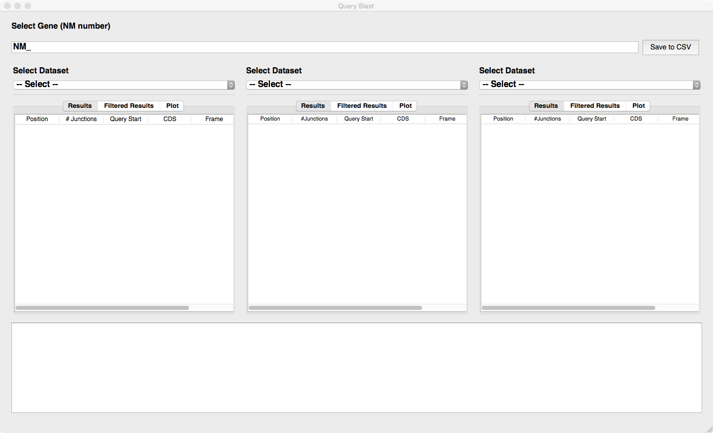
\includegraphics[width=0.8\textwidth]{figure2}
    \caption{Screen shot of Blast Query user interface.}
    \label{fig:blast_query_screen_shot}
\end{figure}


Enter in GeneID in the text box above in Figure \ref{fig:blast_query_screen_shot}.
These are \textbf{NM\_*} identifiers that can be found in relation to gene names in the \texttt{summary.csv} files generated by \GeneCount. An example is \textbf{NM\_146001}.

Then use the pull-down menu to select which datasets to compare. The list of datasets is generated by reading what ``.p'' files are in the \texttt{blast\_results\_query} folder that is within your ``Work Folder''.  If the right .p file is not in that folder, you can simply move it in from somewhere else.


The data window can be selected to display \textbf{Results} , \textbf{Filtered Results} or \textbf{Plot} as shown in Figure \ref{fig:blast_query_screen_shot2}.

\begin{figure}[!ht]
    \centering
    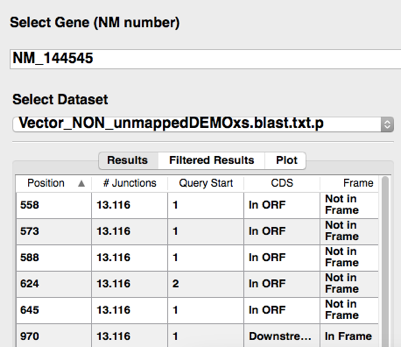
\includegraphics[width=0.8\textwidth]{figure3}
    \caption{Screen shot of Blast Query user interface.}
    \label{fig:blast_query_screen_shot2}
\end{figure}

\begin{remark}
\textbf{Nomenclature for Yeast Open-Reading Frames}.
For most yeast (sacCer3) genes, using the genebank accession numbers is not helpful. Rather, the \emph{Saccharomyces} Genome Database (SGD) uses a different systematic name and also uses common names.  For instance, the genebank entry: NM\_001180490.1 corresponds to the gene having the common name: \emph{CDC1}, which has the SGD systematic name: YDR182W.  \DEEPN uses a custom naming scheme whereby the gene above is designated: \textbf{YDR182W\_CDC1}.  These names are in the \GeneCount Summary .csv file and should be the search term for using \BlastQuery to search through yeast genomic Y2H libraries.  
\end{remark}


\section{Results Tab}\index{Blast Query Results}

The ``Results Tab'' shows

\begin{itemize}
    \item \textbf{Position} (which is the position of first nucleotide of the given insert that found for a particular junction read). 
    \item \textbf{\#Junctions} is a count, in PPM, for how abundant that particular junction is
    \item \textbf{QueryStart} comes from the ``q.start'' value of the \texttt{blastn} search used to identify the downstream gene fused to the Gal4AD.  It refers to how many nucleotides are between the junction tag and the matched cDNA position. Often, this number is 1, but sometimes there are cloning artifacts that generate extra sequence between the end of the Gal4-AD and where the match is to the cDNA.  These extra nucleotides will have an impact on the translation reading frame.  Also, to accomodate the pGAD-C1,-C2,-C3 libraries, the junction sequence is set back a bit from where the insert is positioned, so the q.start is larger. All this means that the \textbf{Position} and the \textbf{QueryStart} are used to calculate whether a particular junction is within the Coding Region (CDS) and whether it is in-frame.
    \item \textbf{CDS} shows whether the junction site in the mRNA of interest is upstream of the coding region, downstream of the coding region, or within (In ORF) of the coding region.
    \item \textbf{Frame} calculates whether the downstream library insert that encodes the candidate protein of interest is in the same frame as the upstream Gal4AD.  Two other values can be returned in this column.  ``Intron'' means that the DNA insert in question could be interrupted by an intron.  This is only a problem with Y2H libraries made from genomic DNA where such things exist.  For instance the pGAD-C1,2,3 libraries made from yeast genomic DNA.  Because of this, \BlastQuery will be agnostic and not calculate whether the candidate gene was actually in frame. ``Backwards'' means that the Downstream Reading Frame is in the opposite orientation.  This is common finding with y2H libraries from genomic DNA, which can go into the plasmid backbone in either orientation.  It is less of an issue with many Y2H cDNA libraries that use a directional cloning strategy.  This ``Backwards'' error is also flagged with a false QueryStart value of ``1000'' 
\end{itemize}

\section{Filtered Results Tab}\index{Blast Query Filtered Results}

Sometimes, sequencing the same junction multiple times leads to sequence errors which can produce reads that have the same \textbf{Position} but different \textbf{QueryStarts}, or that have \textbf{Positions} that are 1-2 bp different from the main \textbf{Position}.  To simplify comparisons, one can use the ``Filtered Results'' tab, which collapses all similar \textbf{Positions} that may have different \textbf{QueryStarts} into a single value. Filtered Results also displays only the \textbf{Positions} that are found within the \textbf{Left} most dataset. Thus, by placing, say, a total unselected library dataset on the left, the \textbf{Right}-hand datasets will only display position sites that are in common with the unselected library dataset.


\section{Plot Tab}\index{Blast Query Plot Tab}

The ``Plot'' tab creates a quick graphic displaying where each junction site is along the given mRNA or gene.  The abundance of each junction sequence within the dataset are plotted on the Y axis in ppm. If a junction site is downstream of the CDS or out of translational frame, the bar is grey.  If it is within the CDS and in-frame it is {\color{RoyalBlue}{dark blue}}, and if it is upstream of the CDS start but within the correct translational reading frame, it is {\color{cyan}{cyan}}.  The start and stop sites for translation are shown with {\color{red}{red}} bars. The mRNA/gene sequence itself is given in the text box below, where the protein coding sequence is shown in black text and the upstream and downstream untranslated regions are in grey.

\section{Export for Graphing}\index{Export for Graphing}

A 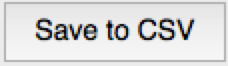
\includegraphics[width=80pt]{Pictures/save_csv_btn} button is found at the top right hand corner.
This will save the current \textbf{Results} and \textbf{Filtered Results} Tables in a \texttt{.csv} file that can be opened in \texttt{Microsoft Excel}. Results from each selected dataset are saved in a different sheet.

This output pasted program for further analysis or graphing such as GraphPad Prism

\vspace{10pt}
\href{http://www.graphpad.com/scientific-software/prism/}{http://www.graphpad.com/scientific-software/prism/}

\chapter{\ReadDepth}\index{Read Depth}

\ReadDepth is used as an aid to determine the 3’ end of the interacting cDNA insert.  Most genes that enrich upon selection are represented by a single plasmid, which can be surmised by having a dominant junction site.  Thus, much of how a given cDNA insert extends downstream can be determined by read-depth along the cDNA sequence. \ReadDepth determines this by measuring how many sequences within the dataset contain a 25 bp interval of the cDNA sequence in question. \ReadDepth first makes a subset of all the mapped reads that correspond to the gene of interest and then counts how many of these reads contain sequence that match along the length of the cDNA. 
The up/down arrows can be used to adjust the interval distance in increments of 50 nt.  Users can also directly enter a desired interval, with a minimum interval of 50~nt.

\begin{figure}[!ht]
    \centering
    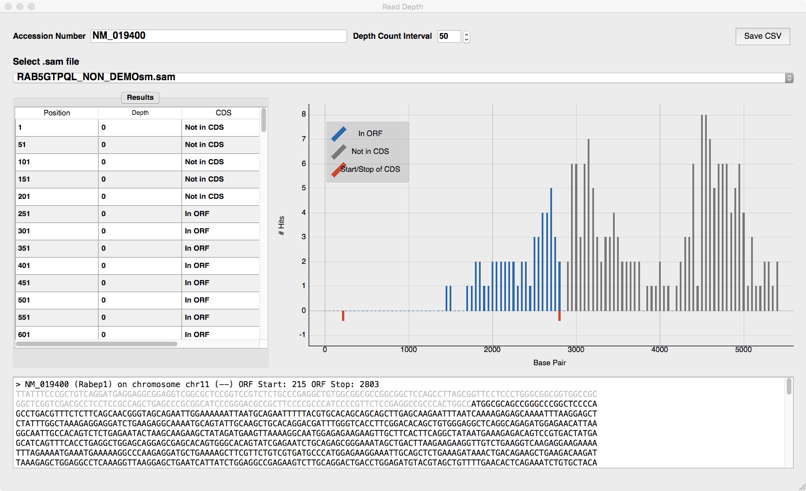
\includegraphics[width=0.8\textwidth]{figure4}
    \caption{Screen shot of Read Depth user interface.}
    \label{fig:blast_query_screen_shot2}
\end{figure}

\cleardoublepage

\part{Appendix}

%----------------------------------------------------------------------------------------
%   CHAPTER 3
%----------------------------------------------------------------------------------------

\chapterimage{chapter_head_1.pdf}

\chapter{Appendix}\index{Appendix}

\section{Experimental Materials}\index{Experimental Materials}

\subsection{Yeast Growth Media}\index{Yeast Growth Media}

\textbf{Yeast Synthetic Defined (SD) Media}

\begin{itemize}
    \item Yeast Nitrogen Base (ammonium sulfate) w/o amino acids (Research Products International; Prospect, Illinois)
    \item Dextrose (2\% final) (Research Products International; Prospect, Illinois)
    \item Supplement

    Adenine (200 mg/l) (Research Products International; Prospect, Illinois), Arginine (20 mg/l) (Research Products International; Prospect, Illinois), Aspartic acid (100mg/l) (Life Technologies; Grand Island, NY), Glutamate monosodium (100mg/l) (FisherScientific, Waltham, MA), Histidine (200mg/l) (Sigma-Aldrich; St. Louis, MO), Leucine (60mg/l) (Sigma-Aldrich; St. Louis, MO), Lysine mono-HCl (30mg/l) (Sigma-Aldrich; St. Louis, MO), Methionine (200mg/l) (Research Products International; Prospect, Illinois), Phenylalanine (50mg/l) (Sigma-Aldrich; St. Louis, MO), Serine (375mg/l) (Sigma-Aldrich; St. Louis, MO), Threonine (200mg/l) (Research Products International; Prospect, Illinois), Tryptophan (200mg/l) (Research Products International; Prospect, Illinois), Tyrosine (30mg/l) (Research Products International; Prospect, Illinois), Valine (150 mg/l) (Research Products International; Prospect, Illinois), Uracil (200 mg/l) (Sigma-Aldrich; St. Louis, MO).  

    \item For plates add 1.5\% Bacto Agar (BD; Franklin Lakes, NJ)
    \item For plasmid or Y2H selection, omit Leucine, Tryptophan, or Histidine as needed
\end{itemize}


\textbf{Yeast Rich Media (YPD)}\index{Yeast Rich Media}

\begin{itemize}
    \item Peptone (20g/l) (Research Products International; Prospect, Illinois)
    \item Yeast Extract (10g/l) (Research Products International; Prospect, Illinois)
    \item Glucose (20g/l)
\end{itemize}

\textbf{Buffered Yeast Rich Media (bYPDA)}

\begin{itemize}
    \item Peptone (20g/l) (Research Products International; Prospect, Illinois)
    \item Yeast Extract (10g/l) (Research Products International; Prospect, Illinois)
    \item Glucose (20g/l)
    \item Adenine (200mg/l)
    \item \emph{adjust PH of above media to 3.7 with HCl, then filter sterilize}
\end{itemize}

\subsection{Reagents}\index{Reagents}

\textbf{TWIRL sample buffer}\index{TWIRL Buffer}

\begin{itemize}
    \item 8M Urea (Research Products International; Prospect, Illinois)
    \item 4\% SDS (Research Products International; Prospect, Illinois)
    \item 10\% glycerol (ThermoFisher, Waltham, MA)
    \item 50 mM Tris-HCl, pH 6.8 (Gibco)
    \item 0.02\% bromophenol blue (Amresco)
\end{itemize}

\textbf{Yeast 2 hybrid library}\index{Yeast-2-Hybrid Library}

\begin{itemize}
    \item Normalized Universal Mouse cDNA library, Mate\&Plate, Cat No: 630483 (Clontech, Mountain View, CA)
\end{itemize}

\textbf{PCR and Cloning}\index{PCR}

\begin{itemize}
    \item Gibson Assembly Master Mix, Cat No: E2611L (New England Biolabs, Ipswitch, MA)
    \item NEBNext High-Fidelity 2x PCR Master Mix, Cat NO: M0541S (New England BioLabs, Ipswitch, MA)
    \item Primers to amplify library inserts of mouse cDNA library in pGADT7:

    \item F1-primer 5’-TCACGGCTAGTAAAATTGATGATGG-3’

    \item R1-primer 5’-GTCCAAAGCTTCTGAATAAGCCCTCG-3’
    \item QIAquick PCR purification kit Qiagen, Cat No: 28104
    \item EcoRI (New England Biolabs, Ipswitch, MA)
    \item BamHI (New England Biolabs, Ipswitch, MA)
\end{itemize}


\textbf{Antibodies}\index{Antibodies}

\begin{itemize}
    \item Monoclonal anti-HA antibodies were purchased from Biolegend; San Diego, CA (cat no: 901514).  Polyclonal anti-myc antibodies were purchased from QED Biosciences Inc.; San Diego CA (cat no: 18826).
\end{itemize}

\textbf{Other Reagents}\index{Other Reagents}

\begin{itemize}
    \item Zymolyase 100T (USBiological; Swampscott, MA; cat no: Z1004) 10mg/ml in Buffer (50mM K2PO4 pH 7.5/50\%Glycerol) stored at -20°C
    \item RNAse A, DNAse protease-free stock (ThermoFisher; Waltham, MA; cat no: EN0531) stored at -20°C
    \item Phenol/Chloroform/Isoamyl alcohol
\end{itemize}

\subsection{Yeast Strains and Plasmids}\index{Yeast Strains and Plasmids}

\begin{itemize}
    \item Y187:  MAT$\alpha$, ura3-52, his3-200, ade2-101, trp1-901, leu2-3, 112, gal4$\Delta$, met–, gal80$\Delta$, URA3::GAL1UAS-GAL1TATA-lacZ.  (Clontech, Mountain View, CA)
    \item PJ69-4A MATa leu2-3,112 ura3-52 trp1-901 his3-200 gal4$\Delta$, gal80$\Delta$, GAL-ADE2 lys2::GAL1-HIS3 met2::GAL7- LacZ   http://depts.washington.edu/yeastrc/
    \item pGBKT7.  Gal4-DNA binding domain expression plasmid. (Clontech, Mountain View, CA)
    \item pGADT7(Gal4-activation domain expression plasmid(Clontech, Mountain View, CA)
\end{itemize}

% %----------------------------------------------------------------------------------------
% %	BIBLIOGRAPHY
% %----------------------------------------------------------------------------------------

 % \chapter*{Bibliography}
 % \addcontentsline{toc}{chapter}{\textcolor{ocre}{Bibliography}}
 % \section*{Books}
 % \addcontentsline{toc}{section}{Books}
 % \printbibliography[heading=bibempty,type=book]
 % \section*{Articles}
 % \addcontentsline{toc}{section}{Articles}
 % \printbibliography[heading=bibempty,type=article]

%----------------------------------------------------------------------------------------
%	INDEX
%----------------------------------------------------------------------------------------

\cleardoublepage
\phantomsection
\setlength{\columnsep}{0.75cm}
\addcontentsline{toc}{chapter}{\textcolor{ocre}{Index}}
\printindex

%----------------------------------------------------------------------------------------

\end{document}